\picturechapter{Human plasma IgG1 repertoires are simple, unique, and dynamic}{Chaptercovers/ch3.pdf} \label{ch-3}
\vspace*{0.25cm}

{\footnotesize Albert Bondt, Max Hoek, Sem Tamara, Sebastiaan C. de Graaf, Weiwei Peng, Douwe Schulte, Danique M.H. van Rijswijck, Maurits A. den Boer, Jean-François Greisch, Meri R.J. Varkila, Joost Snijder, Olaf L. Cremer, Marc J.M. Bonten, Albert J.R. Heck}

\begin{center}
  \vspace{1cm}
  \includegraphics[]{Chapter.3/Figures/ch3a.png}
  \vspace{0.25cm}
\end{center}

\begin{flushleft}
  \vspace*{\fill}
  \rule{\textwidth}{1pt}\\[0cm]
  \textbf{This chapter is based on work in the following publication:}\\
  \footnotesize
  \textbf{\emph{Cell Systems}} (2021), 12:1131-1143, doi:10.1016/j.cels.2021.08.008\\
  \footnotesize
\end{flushleft}
%%Abstract
\begin{abstract102}
  Although humans can produce billions of IgG1 variants through recombination and hypermutation, the diversity of IgG1 clones circulating in human blood plasma has largely eluded direct characterization. Here, we combined several mass-spectrometry-based approaches to reveal that the circulating IgG1 repertoire in human plasma is dominated by a limited number of clones in healthy donors and septic patients. We observe that each individual donor exhibits a unique serological IgG1 repertoire, which remains stable over time but can adapt rapidly to changes in physiology. We introduce an integrative protein- and peptide-centric approach to obtain and validate a full sequence of an individual plasma IgG1 clone \emph{de novo}. This IgG1 clone emerged at the onset of a septic episode and exhibited a high mutation rate (13\%) compared with the closest matching germline DNA sequence, highlighting the importance of \emph{de novo} sequencing at the protein level.
\end{abstract102}
%%Main Text
\thumbforchapter

\section{Introduction}
\lettrine[lraise=0.1, nindent=0em, slope=-.5em]{T}{he}
human immune system protects us not only from threats posed by pathogens but also cancer and various other diseases. The immune response in health and disease is crucially dependent on each person’s repertoire of immune cells, antibodies, and other circulating plasma proteins. A detailed molecular view of these plasma components is crucial to understanding how they affect each individual’s immune response. Immunoglobulins (Igs) represent some of the most important molecules in the human immune system. Ig molecules consist of two identical heavy chains and two identical light chains, held together by a network of disulfide bridges. The heavy chains possess three (IgG, IgA, and IgD) to four (IgM and IgE) immunoglobulin domains with large, conserved regions, which play a role in receptor binding and complement activation. Similar to the heavy chain, the C-terminal domain of the light chain is constant. On the other hand, for both heavy and light chain, the sequence of the N-terminal Ig domains is hypervariable and contains the recognition-determining parts, better known as complementarity-determining regions (CDRs), of the molecule. They are enclosed in the two fragment antigen-binding (Fab) arms of the antibody, consisting of the light chain and the N-terminal parts of the heavy chain (Fd).
The variable regions of the antibody, in particular the CDRs, are optimized to recognize antigens by a process known as affinity maturation. The best antigen binders, modified through somatic recombination and hypermutation of numerous coding gene segment variants, give rise to the mature IgG secreting plasma B cells that produce the antibodies that end up in our circulation. The circulating antibodies, thus, consist of the fully matured heavy- and light-chain variable domain sequences that harbor the CDRs, joined by generally less sequence-variable framework regions (FR). Each unique combination of mature chains is called an Ig clone.
Considering the genes encoding the variable domain sections and the known genomic rearrangements, somatic hypermutations, and post-transcriptional processes that join these sections—resulting into the ultimate protein products—it has been estimated that in humans the theoretical molecular Ig diversity may extend beyond 10\textsuperscript{15} \cite{schroeder2006similarity}. Not all theoretically possible Ig clones will be expressed in the human body, since the number of B cells in a human body is several orders of magnitude lower (1–2 × 10\textsuperscript{11}) \cite{apostoaei2012review}. Nevertheless, it has been assumed that the actual repertoire of circulating Igs is extremely large and diverse \cite{briney2019commonality, soto2019high}.
Recombinantly expressed clones (mainly IgG) have become a major class of therapeutics, used to fight multiple types of pathologies such as cancers and various infectious diseases. Recent developments have moved the field toward using therapeutic monoclonal antibody (mAb) sequences derived from human subjects instead of laboratory animals; this trend is exemplified by successful new treatments for Ebola \cite{corti2016protective, dyer2019two, mulangu2019randomized} and COVID-19 \cite{jones2021neutralizing}. These therapeutic antibody sequences are inferred from genetic material recovered from patients that successfully overcame the disease. The ability to detect and identify individual mature IgG protein sequences directly from donor specimens would aid such efforts.
To experimentally determine the Ig repertoire, attempts have been made to sequence Ig nucleic acids from bulk B cell populations or B cell subsets from single donors. These Igs are analyzed with high-throughput sequencing (Ig-seq or Rep-seq) at the DNA or RNA level \cite{georgiou2014promise}, resulting in datasets of tens to hundreds of thousands of unique reads of variable abundance \cite{vollmers2013genetic}. Unfortunately, these analyses at the level of DNA and RNA do not measure the actual antibodies of interest, and the presence of a cognate BCR sequence in the B cell population provides no information regarding abundance levels of the antibodies that end up in circulation.
Alternatively, the challenge could be approached from the protein level, analyzing the Ig repertoire present in circulation. The most abundant Ig in human plasma is IgG, at a concentration of approximately 10 mg/mL during health \cite{cassidy1975human, gonzalez-quintela2008serum}. Of the four IgG subclasses, IgG1 is the most abundant, accounting for more than 50\% of all IgGs \cite{giessen1975quantification} in most people. Given the extremely high theoretical limits on Ig diversity and the large number of experimentally determined variants, most researchers have refrained from analyzing plasma antibodies directly at the protein level. It has been mostly assumed that it is impossible to detect any single Ig clone against the expected background of thousands to millions of other clones.
However, in recent years, several attempts have been made to identify plasma Igs directly. G. Georgiou and colleagues should be considered pioneers. In their method (also referred to as Ig-seq, but protein-based instead of solely gene-based), IgGs are purified from plasma, and tryptic Ig peptides are characterized using liquid chromatography coupled online to tandem mass spectrometry (LC-MS/MS), focusing on the detection of IgG heavy-chain CDR3 peptides \cite{chen2017proteomic, lavinder2014identification, lee2016molecular-level, lee2019persistent, wine2013molecular}. Another recently developed proteomics approach uses LC-MS to profile intact light chains purified from plasma \cite{barnidge2014phenotyping, barnidge2014using, he2019classification, he2017analysis, mills2015detecting, sharpley2019novel}. In another report, profiling and sequencing of intact Fabs was attempted, but the sensitivity was too low, and only a few sequence tags could be derived from separated light chains \cite{wang2019top-down}.
In these approaches, information about the heavy- and light-chain pairing is often lost, which is unfortunate as only the combined CDRs from both heavy and light chain provide the full complementarity against an antigen. Of note, in nearly all these studies, only a subset of plasma immunoglobulins recognizing and binding a specific antigen was targeted, or a mAb spiked into plasma was used as a model. Nevertheless, the remarkable observation was made that a person’s plasma Ig repertoire could be several orders less variable than assumed based on the available B cell repertoire and likely dominated by only a limited number of clones. Whether this observed number of IgGs is a consequence of the targeted analysis of antigen-specific IgGs or diseases with monoclonal IgG overexpression (gammopathy) remained unclear.
Here, we introduce a sensitive and efficient approach for quantitative plasma IgG1 clone profiling. The method was applied to a sample set of two healthy control donors, as well as eight critically ill patients, from which sequential plasma samples were retrieved while developing nosocomial sepsis, experiencing a dramatic immunological change in a relatively short time span (\textbf{\autoref{fig:fig3.1}a}). The application of our method revealed several important properties of the human plasma IgG1 repertoire: (1) the total IgG1 repertoire is dominated by a few dozen clones, but (2) is unique for each individual, and (3) single clones are differentially affected by physiological changes. Next, as proof of concept, we \emph{de novo} sequenced a single plasma clone—that appeared at sepsis onset—directly from human plasma, only made possible by using iteratively a combination of protein-centric and peptide-centric proteomics. To validate the correctness of the derived \emph{de novo} IgG1 sequence, we produced its recombinant mAb equivalent and compared its key structural features with the plasma clone. We foresee that this approach will unlock the potential of mass spectrometric analysis and identification of disease-responsive IgGs that may be directly evaluated and used as therapeutic agents, as they do already represent fully matured, fully human Abs.
\begin{figure*}[!htb]
  \center
  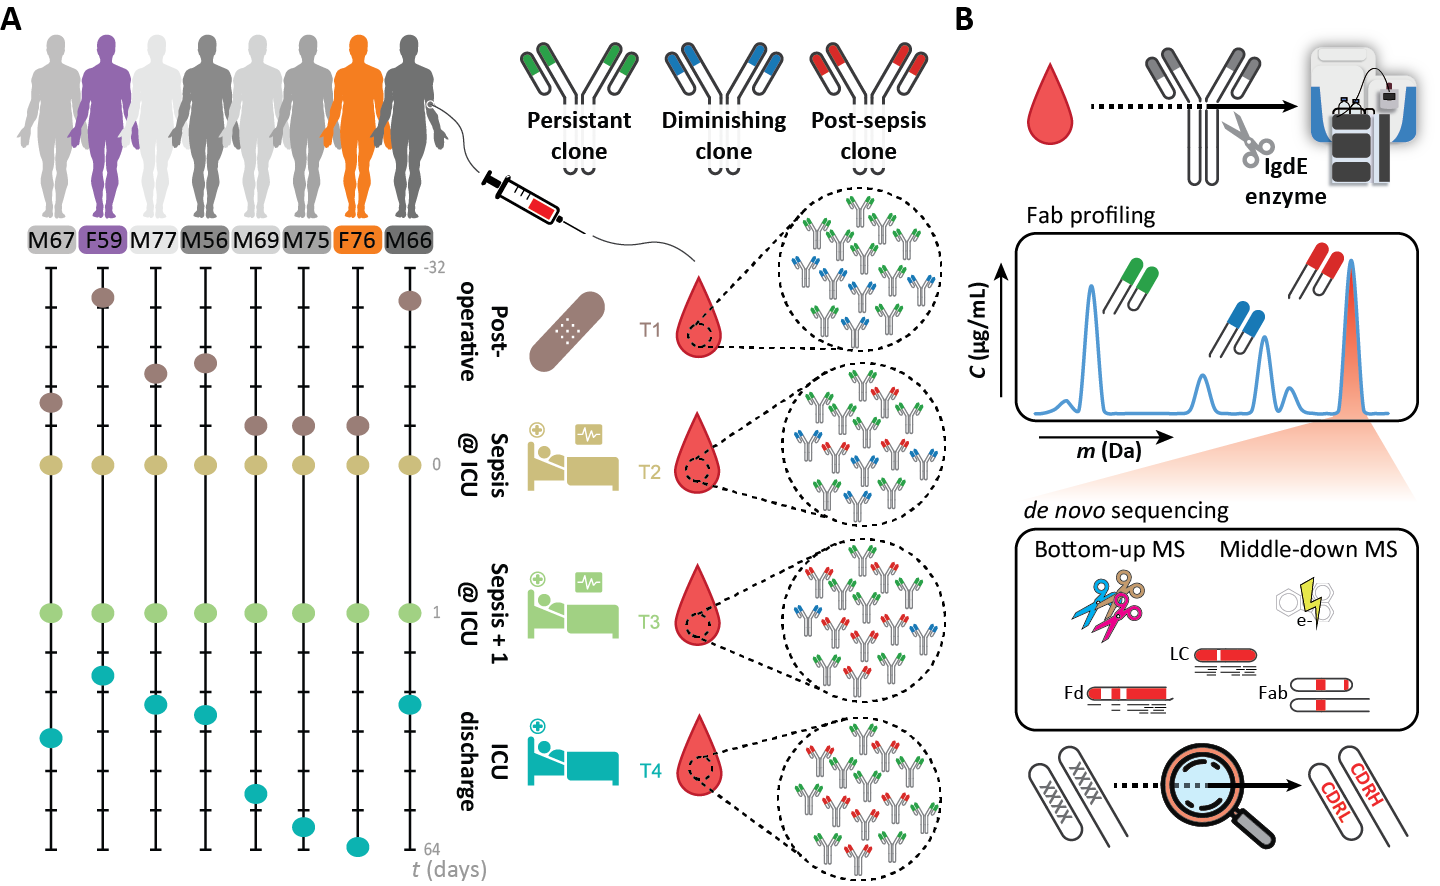
\includegraphics[]{Chapter.3/Figures/f1.png}
  \caption{
    \textbf{Monitoring individual plasma IgG1 profiles.} ~~a) Longitudinal analysis of the IgG1 repertoire from sepsis patient plasma obtained at four time points, reveals its simplicity and clonal dynamics: some clones are fairly constant (green), some disappear (blue), whereas others appear over time (red). ~~b) The experimental approach taken involves IgG capturing from 10–100 μL of serum, followed by the specific enzymatic digestion of the IgG1 molecules in their hinge region, generating two identical Fab portions. All generated Fabs are collected and subsequently subjected to LC-MS analysis. The clonal repertoire is profiled, whereby each identified clone is characterized by its unique mass and retention time. A single post-sepsis clone from one of the patients (F59) was selected for \emph{de novo} sequencing, combining protein- and peptide-centric mass-spectrometry-based sequencing. The extracted full sequence of the plasma IgG1 was validated by analyzing, in a similar manner, a recombinant IgG1 analog of the plasma clone.
  }
  \label{fig:fig3.1}
\end{figure*}


\section{Results}

\subsection{Mass-spectrometry-based Fab profiling of the human plasma repertoire}
To chart and monitor the nature of the plasma IgG1 repertoire, we started our analysis with 10 μL of plasma, derived from a single donor. From such a sample, we first captured all intact IgGs using affinity beads. Subsequently, the captured IgG molecules were digested using the highly specific Ig degrading enzyme (IgdE), cleaving specifically IgG1’s at a defined site in the upper hinge region, resulting in the segregated Fc (that remains bound to the affinity beads) and two identical Fabs (\textbf{\autoref{fig:fig3.1}b}) \cite{spoerry2016novel}. We focused on the Fab fragments derived from the intact IgGs because this (1) concentrates the clonal signal since each IgG1 provides two identical Fab molecules, (2) results in more homogeneous mass profiles by removing the Fc portions that harbor two heterogeneous N-glycosylation sites, and (3) retains all hypervariable CDRs, which define the unique identity and antigen recognition of each clone.
Following elution of the IgG1 Fabs, all these intact 45–53-kDa Fab molecules were subjected to reversed-phase LC-MS. All individual Fab fragments were subsequently characterized by their distinctive mass and chromatography retention time. In our analyses, we spiked-in two monoclonal IgG1 antibodies (\textbf{Data \ref{tab:tabdummy3.1}}, mAbs \#1 and \#2) of known sequence at a defined concentration. These mAbs were used as internal standards for mass and retention time calibration and quantification of all the other distinctive plasma IgG1 clones. This also allowed us to calculate the precision and accuracy of retention time, mass, and quantification in our measurements as illustrated in \textbf{\autoref{fig:figs3.1}a}.
Using a mixture of six monoclonal antibodies (\textbf{Data \ref{tab:tabdummy3.1}}) spiked into a single-donor plasma background, we furthermore observed linear relationship between (1) the quantity of mAbs that were spiked into the plasma sample, and (2) the quantity that is observed (R\textsuperscript{2} = 0.99, \textbf{\autoref{fig:figs3.1}b}), using a dilution/titration with 4,000, 800, 200, and 20 ng per mAb. Of note, no discrepancy was observed for the Fab glycosylated mAb as compared to the other mAbs. To evaluate the repeatability (technical replicate and sample preparation replicate), the 100 most abundant plasma-derived clones in this sample were quantified in multiple replicates (\textbf{\autoref{fig:figs3.1}c}). Finally, one of the samples was injected three times to serve as injection replicates (\textbf{\autoref{fig:figs3.1}c}, \#1). From all these validation experiments, we concluded that, by using the approach depicted here (\textbf{\autoref{fig:fig3.1}}), the repertoire of Fab clones could be accurately and reproducibly determined from as little as 10 μL of plasma obtained from a single donor at a single time point.

\subsection{Plasma IgG1 repertoires are dominated by a few clones}
Next, we analyzed in parallel a set of 32 plasma samples obtained from eight patients of the Dutch molecular diagnosis and risk stratification of sepsis (MARS) cohort (\textbf{\autoref{fig:fig3.1}a}; \textbf{Data \ref{tab:tabdummy3.2}}). All these patients underwent major gastrointestinal surgery and subsequently developed an infectious complication (i.e., anastomotic leakage or pneumonia) resulting in sepsis. Plasma samples were obtained from the patients at four different stages: within 24 h of surgery when no signs of sepsis were present (sample T1; between t = −19 and t = −2 days), on two consecutive days after onset of sepsis (samples T2 and T3; t = 0 and t = 1 day), and upon intensive care unit (ICU) discharge, when the sepsis had been resolved (sample T4; between t = 3 and t = 61 days) (\textbf{\autoref{fig:fig3.1}a}). In addition, to monitor the nature of the plasma IgG1 repertoire in healthy donors, we performed an identical analysis on two sets of three sequential healthy donor plasma samples, each collected roughly 1 month apart.
In marked contrast to expectations of extensive IgG1 diversity, we observed that all the LC-MS profiles of IgG1 Fab molecules were dominated by just a few dozen peaks, both in the 32 sepsis plasma samples as well as in the six plasma samples of the healthy donors (\textbf{Data \ref{data:datadummy3.1} and \ref{data:datadummy3.2}}). In each of the LC-MS runs, we could pick up distinctive IgG1 signals of between 35 and 543 in abundance dominant clones (median 196; \textbf{Data \ref{data:datadummy3.1}}) that we distinguished by their masses in Dalton and retention times (RT) in minutes. Each detected clone was given a unique identifier: \textsuperscript{RT} \# \textsubscript{mass}.
We found that the summed concentrations of the 30 most abundant IgG1 clones account for more than two-thirds of all IgG1 molecules detected from plasma (median 71.8\%, range 47.3\%–98.3\%, \textbf{Data \ref{data:datadummy3.1}}). The full lists of detected clones are provided in \textbf{Data \ref{data:datadummy3.1}}. In addition, the deconvoluted mass plots (similar to \textbf{\autoref{fig:fig3.2}c}) and the raw chromatograms supported by extracted chromatograms for all identified Fabs obtained in the LC-MS measurements are provided in \textbf{Data \ref{data:datadummy3.2}}, and one example of the actual raw mass spectrometry data of Fabs that we have analyzed is provided in \textbf{Data \ref{data:datadummy3.3}}.


Next, we looked at the cumulative mass distribution of all detected IgG1 Fabs in the plasma samples from all donors and at all time points. This cumulative mass distribution—representing more than 5,500 clones experimentally identified—resembled the expected mass distribution of over 130 million IgG1 Fabs constructed from the sequences in the ImMunoGeneTics information system (IMGT) \cite{lefranc1999imgt} database (\textbf{\autoref{fig:figs3.1}d}), revealing that we profiled a representative IgG1 repertoire.

\begin{figure*}[!hp]
  \center
  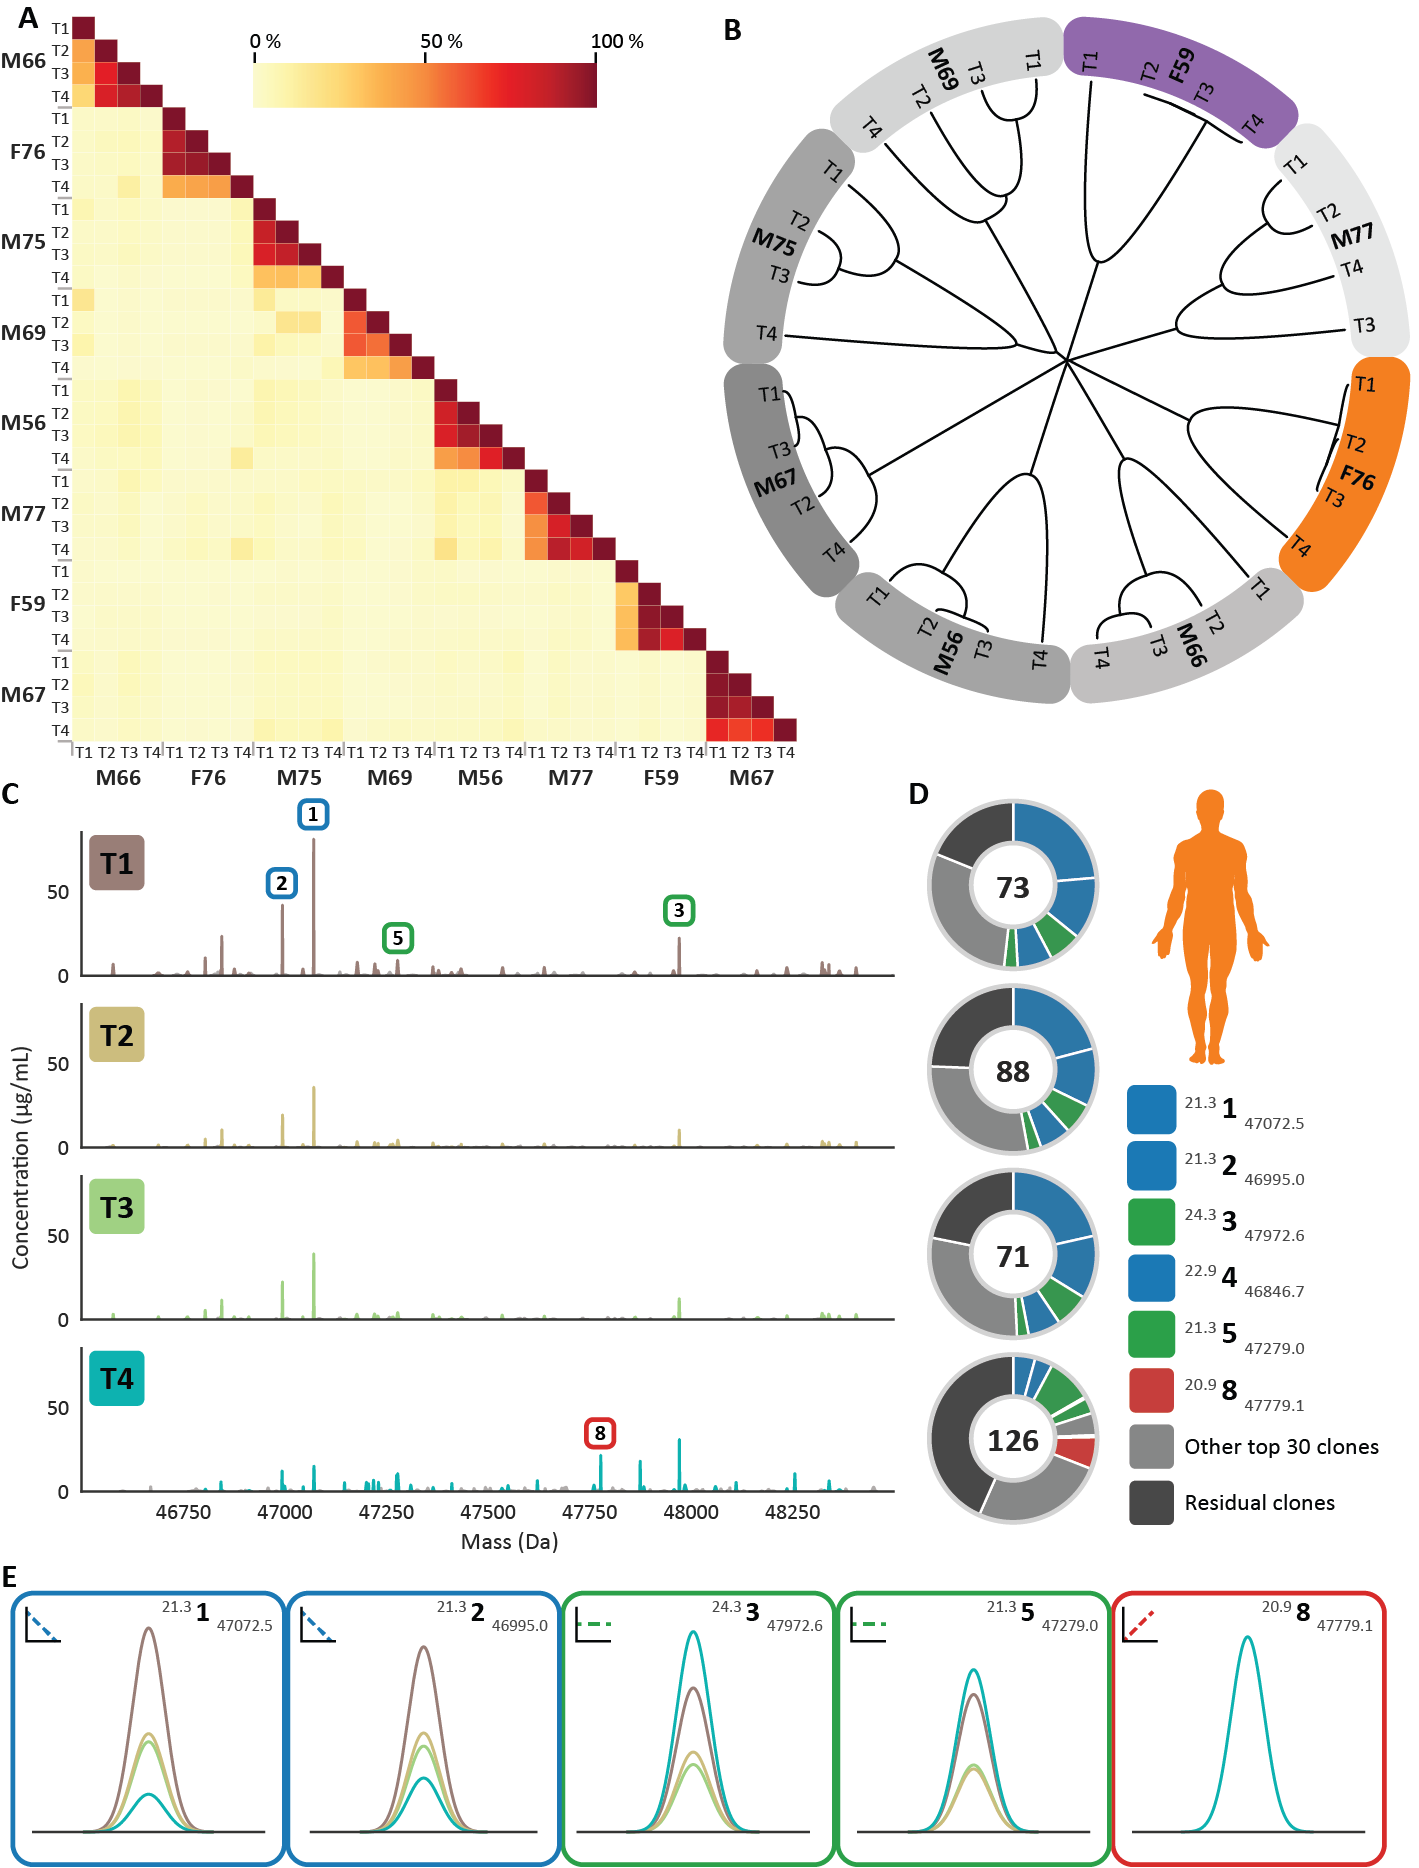
\includegraphics[]{Chapter.3/Figures/f2.png}
  \captionsetup{singlelinecheck = false, format= hang}
  \caption{
    Figure legend on next page.
  }
  \label{fig:fig3.2}
\end{figure*}
\addtocounter{figure}{-1}
\begin{figure*}[!ht]
  \caption{
    \textbf{Monitoring personalized plasma Fab repertoires reveals not only their simplicity and extreme donor uniqueness but also longitudinal clonal variations within a single donor.} ~~a) Heatmap illustrating the degree of overlap between the detected IgG1 repertoires in all analyzed sepsis patient plasma samples. For each of the eight donors, four sampling times were available, and Fab profiles were measured by LC-MS analysis. Each LC-MS peak, exhibiting a unique mass and retention time pair, was considered a unique clone and annotated as \textsuperscript{RT} \# \textsubscript{mass}. The amount of Fab molecules, based on intensity that is persistent, is quantified and shown as a percentage as indicated by the color bar. In between donors, the overlap is found to be on average 3\%, whereas within a single donor at different time points the overlap was found to be in between 26\% and 98\%. ~~b) Hierarchical clustering of the Fab clonal repertoires based on correlation distance. The branch lengths depict the distance between the repertoires. Donors are colored as in \textbf{\autoref{fig:fig3.1}a}. ~~c) Longitudinal deconvoluted Fab mass profiles of donor F76 at each of the four time points. Each peak represents a unique Fab at its detected mass and plasma concentration. The top 30 most intense Fab clones in each sample are colored reflecting the time points, the other clones are colored gray. Five peaks are highlighted with a box that is colored based on the longitudinal behavior of the Fab concentration in plasma (blue, diminishing clone; green, persistent clone; and red, post-sepsis clone), a magnified version of each of these Fab signals is shown in ~~e) . ~~d) Pie charts portraying the total number and distribution of clones in donor F76 for each time point. The value within the chart displays the number of identified unique Fab molecules. The five most intense Fabs are colored based on longitudinal behavior, and their mass and retention time are depicted in the legend in order of abundance. ~~e) Magnified mass plots for each of the highlighted clones. The peaks are colored according to the time points, the surrounding border and sign indicate the longitudinal behavior and the top right shows the annotated clone ID.
  }
\end{figure*}

As can be seen in \textbf{\autoref{fig:figs3.1}d}, most Fab fragments exhibit masses between 46 and 49.5 kDa. However, we also did detect some higher Fab masses, which may be indicative of Fab glycosylation. The average mass of Fab glycans is estimated to be around 2,300 Da \cite{bondt2016fab, hafkenscheid2017structural}. In two of our donors, annotated M66 and M77, we did detect relatively high levels of Fab glycosylation as shown for M66, time point 3, in \textbf{\autoref{fig:figs3.2}a}, with the annotation of the putative Fab glycosylation annotated in \textbf{\autoref{fig:figs3.2}b}. Still the Fab glycosylated clones represented just a few percent of the total abundance (2\%–6\% for donor M66 and M77). The fractional abundance of glycosylated Fabs in the other patients was between 0\% and 1.86\% (with a median of 0.295\%) (\textbf{\autoref{fig:figs3.2}c}). Also, in the two healthy donors, one displayed a fractional abundance of glycosylated Fabs of about 3\% (F66H), whereas in the other donor this remained around 0.5\% at all sampling time points. This fractional abundance is substantially lower than would be predicted based on the IMGT database ($\sim$11\% of these 130 million sequences carry at least one consensus N-glycosylation site) and lower than the $\sim$17\% described in literature \cite{bondt2016fab, hafkenscheid2017structural}. However, our data reveal that the fractional abundance of glycosylated Fabs is also donor-dependent.

\subsection{Plasma IgG1 repertoires are unique for each donor}
Next, we compared the IgG1 Fab profiles between time points not only within a single donor but also between different donors. Interindividual analyses showed that virtually none of the Fab IDs overlapped between individuals (\textbf{\autoref{fig:fig3.2}a, \autoref{fig:figs3.3} and \autoref{fig:figs3.4}a and b}). Also, hierarchical clustering based on clone IDs clusters each donor distinctively (\textbf{\autoref{fig:fig3.2}b}). Thus, each donor has its own simple albeit unique IgG1 repertoire. However, within each individual, overlap between the measured IgG1 repertoires measured across time was found to be very high, even when the time span largely exceeded the average half-life of IgG1s (\textbf{\autoref{fig:fig3.2}a–d and \autoref{fig:figs3.4}}). A large portion of the most abundant IgG1s remains present throughout the sampling window of up to 2 months, although we also observe a response in the IgG1 profile due to changes in the patient’s physiology (discussed below). To exclude whether these findings were due to the severe physiological state of the eight septic patient donors, we performed a similar analysis on plasma of two healthy donors. In the absence of a dramatic immunological challenge, the IgG1 profiles, as obtained from the two healthy donors, show (1) a very high stability over time within individuals and (2) an interindividual overlap in uniquely RT- and mass-identified IgG1 clones near to zero (\textbf{\autoref{fig:figs3.4}a and b}).

\subsection{Longitudinal quantitative monitoring of single IgG1 clones}
By spiking in two recombinant IgG1 mAbs at a known concentration to the plasma samples prior to sample preparation, we could provide additional absolute quantification for the abundance of the detected IgG1s. The concentrations of the LC-MS-detected endogenous IgG1 clones present in plasma ranged from less than 0.05 up to >400 μg/mL (<300 pM up to >2.5 μM, median $\sim$6.25 nM; \textbf{Data \ref{data:datadummy3.1}}). Monitoring serological IgG1 repertoires over time in patients who had undergone a septic episode, we observed several distinct quantitative patterns. The most recognizable patterns are highlighted in \textbf{\autoref{fig:fig3.2}c–e}. There are IgG1 clones that become lower in concentration over time (\textbf{\autoref{fig:fig3.2}c–e}, blue boxes). Another category of IgG1 clones was undetectable in the plasma until post-sepsis but became abundantly present at T4 (\textbf{\autoref{fig:fig3.2}c–e}, red boxes). Yet, another group of IgG1 clones was found to be rather persistent in concentration over all sampling moments (\textbf{\autoref{fig:fig3.2}c–e}, green boxes). In healthy donors, the majority of clones were more persistent in concentration, although some subtle changes could be observed for some clones.

\subsection{Full \emph{de novo} sequencing of an individual plasma IgG1 clone}
From the data presented earlier, we can conclude that the plasma IgG1 repertoire of individual healthy and diseased donors is unique and dominated by a few dozen abundant clones. Next, we sought to identify the exact sequences of these clones to obtain further insight into their function and origin. Complete \emph{de novo} sequencing of serological IgGs is notably difficult for several reasons. First, the inherent sequence hypervariability has so far proven to be highly challenging even when (personalized) genome-based sequence templates are available. Second, \emph{de novo} sequencing of antibodies at the protein level by MS is hampered by the complex nature of IgG molecules, stemming from their multichain structure and the intricate network of disulfide bridges. Finally, although shotgun proteomics can be used to obtain (partial) sequences of purified mAbs \cite{guthals2017de, sen2017automated, tran2016complete}, this becomes several orders of magnitude more difficult in a plasma background containing many IgG molecules of closely homologous sequences.
To tackle this challenge, we explored a hybrid and iterative approach combining state-of-the-art peptide-centric (i.e., bottom-up) and protein-centric (i.e., middle-down) mass-spectrometric sequencing methods, using dedicated algorithms to mix-and-match the extracted proteomics-based sequencing data. As proof of concept, we attempted to fully sequence the light and heavy chain of a Fab derived from a single highly abundant IgG1 clone observed in donor F59. This donor showed a plasma IgG1 repertoire dominated by two clones in particular: \textsuperscript{24.4} 1 \textsubscript{47,359.4} (average mass 47,359.4 Da, retention time 24.4 min) and \textsuperscript{20.6} 2 \textsubscript{47,025.7} (\textbf{\autoref{fig:fig3.3}a}). We focused on the \textsuperscript{24.4} 1 \textsubscript{47,359.4} clone, as this clone appeared exclusively after the onset of sepsis.

\begin{figure*}[!hptb]
  \center
  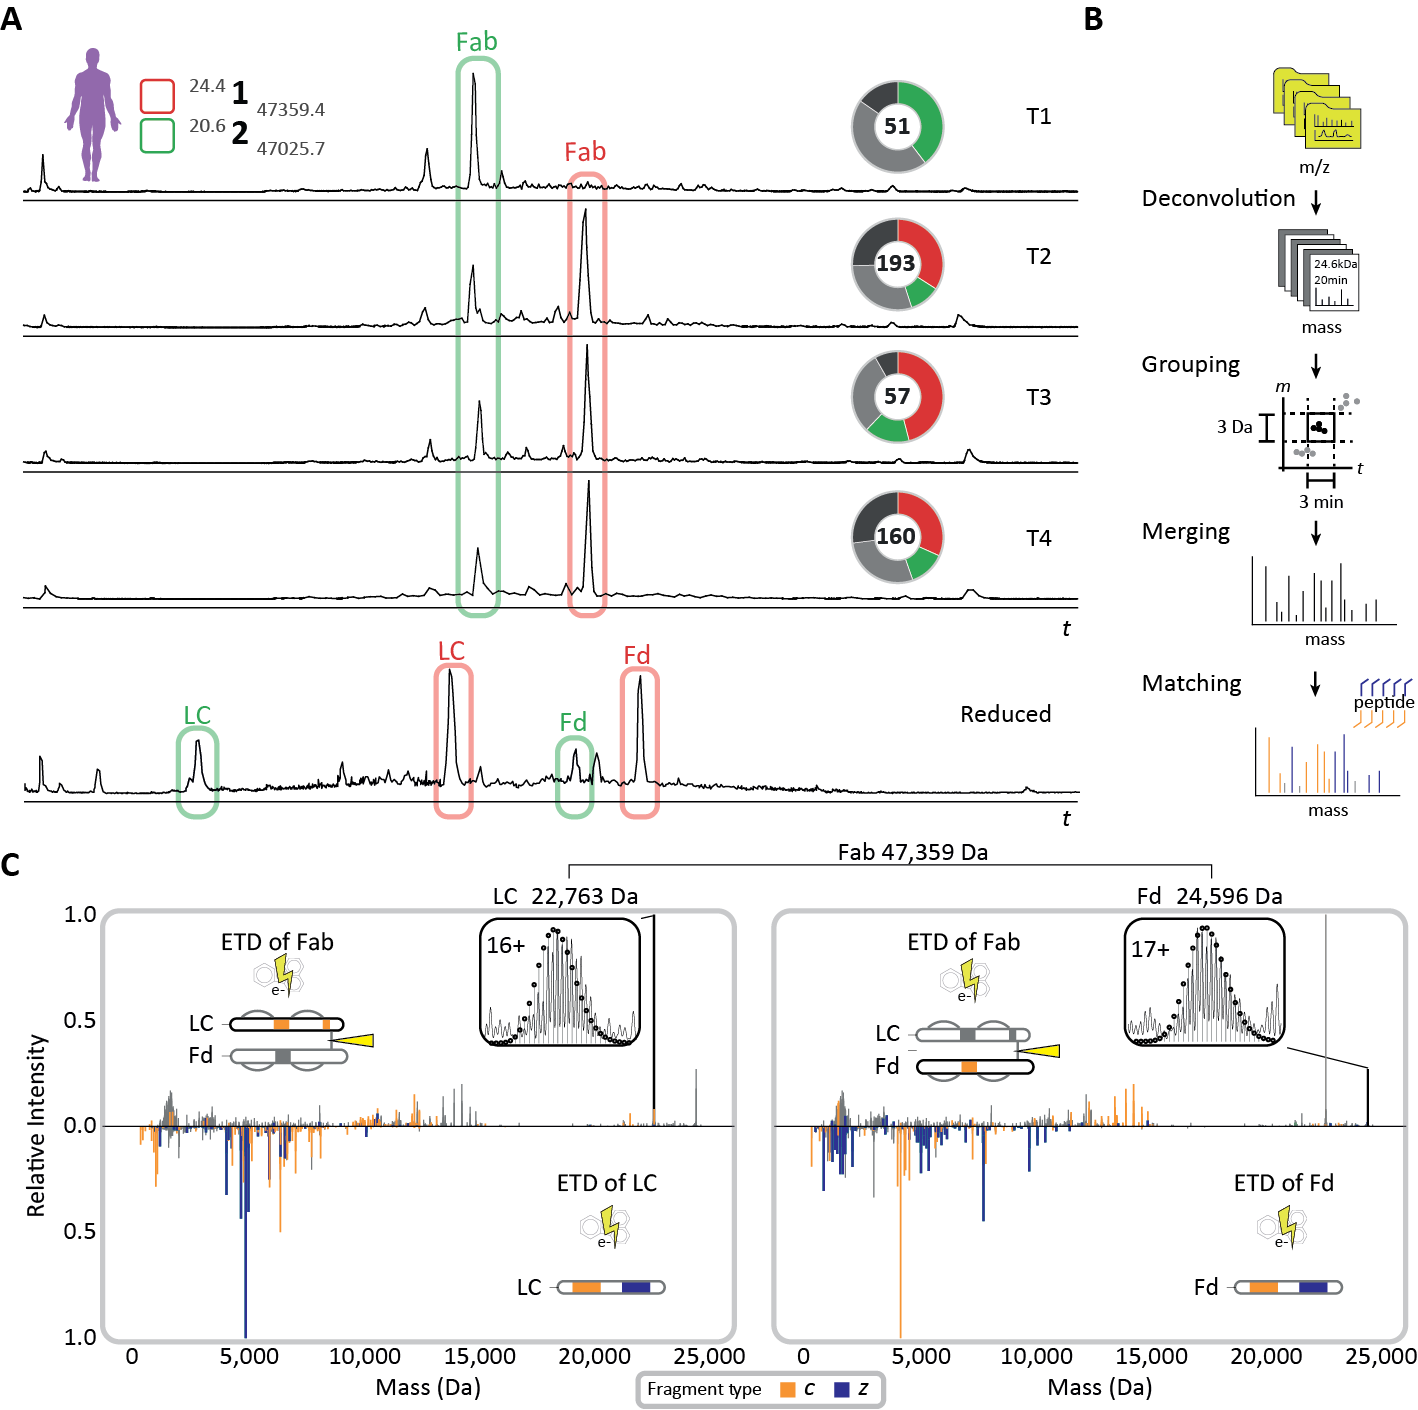
\includegraphics[]{Chapter.3/Figures/f3.png}
  \caption{
    \textbf{Middle-down sequence characterization of the Fab clone \textsuperscript{24.4} 1 \textsubscript{47,359.4} that becomes dominant in the repertoire after the onset of sepsis—under reducing and non-reducing conditions.}
    ~~a) Reversed-phase LC-MS base peak profiles of the Fab repertoire detected in samples T1-4 from donor F59 (top 4 profiles) reveal the dominance of a small number of clones, whereby especially clone \textsuperscript{24.4} 1 \textsubscript{47,359.4} becomes dominant in abundance after the onset of sepsis. The LC-MS chromatogram of the reduced and denatured Fab repertoire from donor F59 at T3 is depicted in the bottom panel. The light chains (LCs) and the N-terminal portions of the heavy chains (Fd) of the two dominant clones are annotated with corresponding colors and chain names. All species highlighted in red were subjected to middle-down LC-MS/MS using ETD. ~~b) Data processing workflow to prepare middle-down ETD-MS/MS spectra for fragment matching and sequence-tag detection (see Methods section for details). ~~c) Deconvoluted ETD-MS/MS spectra of the intact Fab (top spectra) and reduced LC and Fd fragments thereof (mirrored spectra) with the c/z-fragment ions annotated for the LC (left) and Fd (right). The isotopic envelopes of the most abundant charge states of the LC and Fd fragments released from the Fab upon ETD are depicted in the insets with theoretical isotope distributions of the corresponding chain sequences overlaid as black circles. Masses of the LC and Fd fragments and the cumulative mass of the Fab are indicated above the spectra. See also \textbf{\autoref{fig:figs3.6}} for more detail on the fragment ions identified in these middle-down MS spectra.
  }
  \label{fig:fig3.3}
\end{figure*}

Following fractionation and selection of the \textsuperscript{24.4} 1 \textsubscript{47,359.4} clone, we subjected this Fab to mass-spectrometry-based \emph{de novo} sequencing, combining data from middle-down and bottom-up proteomics (\textbf{\autoref{fig:fig3.1}b}). The \emph{de novo} sequence information from both approaches was used to first select several closely matching light- and heavy-chain templates from the publicly available IMGT database of IgG germline sequences (\textbf{\autoref{fig:figs3.5}; \autoref{tab:tabdummy3.3} and \autoref{tab:tabdummy3.4}}). Subsequently, the bottom-up and middle-down sequencing data and the measured intact accurate masses of the Fab, light chain, and Fd were used to refine the selected template sequences and ultimately determine the mature sequence present in the donor, revealing discrepancies between the germline and mature sequences.
In the protein-centric approach, we performed electron transfer dissociation (ETD) on the intact Fab, as well as the light chain and Fd separately, obtained by reduction of the Fab molecule (\textbf{\autoref{fig:fig3.3}a}, bottom trace). Several fragmentation scans obtained for the intact Fab, the separated light chain, and Fd were grouped and combined based on their unique precursor mass and retention time (\textbf{\autoref{fig:fig3.3}b}). The ETD mass spectra of the intact Fab yielded accurate masses of the light chain and Fd by cleavage of the interchain disulfide bond, thus providing direct information about the light-chain-heavy-chain pairing (\textbf{\autoref{fig:fig3.3}c}, top spectra). In addition, these ETD spectra yielded extended sequence tags, covering informative parts of the CDR3 and framework (FR) 4 regions of both Fab chains, in a similar manner as previously reported by performing ETD or ECD of intact IgG molecules \cite{boer2020selectivity, fornelli2017top-down, shaw2020direct}. Complementary, ETD spectra of the separated Fab chains yielded partial sequence information for the FR1, CDR1, FR2, CDR2, and the constant region of the selected clone (\textbf{\autoref{fig:fig3.3}c}, bottom spectra and \textbf{\autoref{fig:figs3.6}}). Although our middle-down MS data provided valuable information about the clone of interest, they did not fully cover the sequence, primarily due to incomplete fragment formation and ambiguous sequence information obtained from the larger fragments.
To further extend our sequencing attempt, we subjected the fraction containing the targeted IgG1 clone to enzymatic digestion, using in parallel four proteases: trypsin, chymotrypsin, thermolysin, and pepsin. The resulting peptides were analyzed by a bottom-up approach, using \emph{de novo} sequencing algorithms for sequence annotation \cite{peng2021mass}. Although fractionated and enriched for the desired \textsuperscript{24.4} 1 \textsubscript{47,359.4} clone, the bottom-up MS data also contained numerous peptides originating from co-isolated plasma clones (\textbf{\autoref{fig:figs3.7}}), which made it impossible to determine the correct sequence by solely using the bottom-up MS data. Nevertheless, by iteratively extending the sequence information from the middle-down MS approach with the \emph{de novo} peptides from the bottom-up MS approach, we ultimately were able to extract the most likely germline precursor of the targeted clone and, notably, its mature sequence by implementing various single-amino-acid mutations not present in the IMGT database (\textbf{\autoref{fig:fig3.4}}).
\begin{figure*}[!hptb]
  \center
  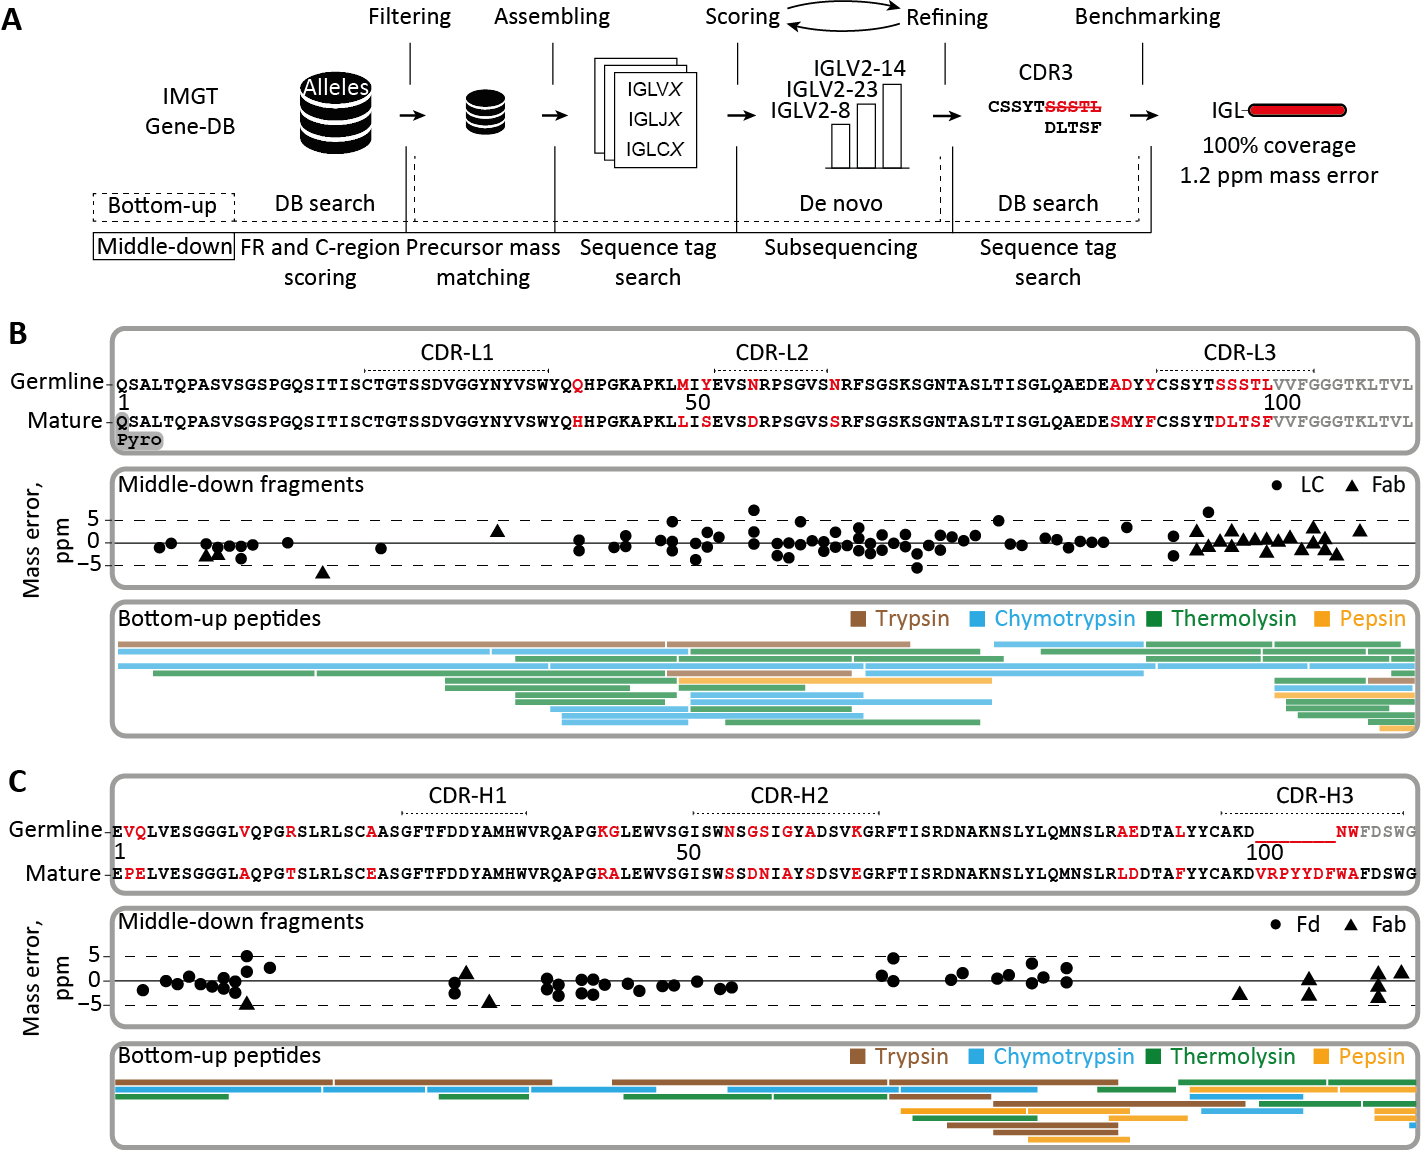
\includegraphics[]{Chapter.3/Figures/f4.png}
  \caption{
    \textbf{Integrative \emph{de novo} sequencing of the Fab clone \textsuperscript{24.4} 1 \textsubscript{47,359.4} from donor F59 combining middle-down and bottom-up MS data.} ~~a) Data analysis pipeline displaying the key steps in the \emph{de novo} sequencing, namely, filtering of the germline database of light- and heavy-chain sequences, assembling of selected allelic variants with mass constraints, scoring of the assembled sequences by using middle-down MS data, iterative refining of the best scoring templates by using peptides in bottom-up MS, and benchmarking of the optimized mature sequences using data from both middle-down and bottom-up MS analysis. ~~b) Alignment of the best matching germline IGLV amino acid sequence from the IMGT database (IGLV2-14$\star$01) with the mature sequence that was determined for the light chain of the dominant clone (top box), the fragments from middle-down MS (middle box), and the peptides from bottom-up MS. ~~c) Alignment of the best matching germline IGHV amino acid sequence from the IMGT database (IGHV3-9$\star$01) with the mature sequence that was determined for the Fd of donor F59’s clone \textsuperscript{24.4} 1 \textsubscript{47,359.4} (top box), the fragments from middle-down MS (middle box), and the peptides from bottom-up MS. CDR regions in top panels of ~~b) and ~~c) were annotated with reference to the closest matching IMGT sequence. Amino acids that were determined to be different in the mature \textsuperscript{24.4} 1 \textsubscript{47,359.4} sequence are highlighted in red.
  }
  \label{fig:fig3.4}
\end{figure*}

In more detail, by using the IMGT database of germline sequences as input, the cumulative MS evidence revealed that the analyzed IgG1 Fab carried a lambda light chain. This light chain originated from a combination of the immunoglobulin lambda (IGL) variable (V) 2-14$\star$01 (IMGT/LIGM-DB: Z73664), IGL joining (J) 2$\star$01 (IMGT/LIGM-DB: M15641), and IGL constant (C) 2$\star$01 (IMGT/LIGM-DB: J00253) alleles. For the heavy-chain Fd portion, we determined that it was constructed from the immunoglobulin heavy (IGH) V3-9$\star$01 (IMGT/LIGM-DB: M99651), IGHJ5$\star$01 (IMGT/LIGM-DB: J00256), and IGHG1$\star$03 (IMGT/LIGM-DB: Y14737) alleles and a diversity (D)-region, which substantially deviated from any reported germline D-region. Although initial identification resulted in just a partial sequence coverage, we could fill the gaps in the germline sequences using sequence tags from the middle-down MS and the \emph{de novo} peptides from the bottom-up MS (\textbf{\autoref{fig:figs3.8} and \autoref{fig:figs3.9}}). Eventually, our approach resulted in a complete and exact precursor mass match for the light and heavy chains, 100\% sequence coverage in bottom-up MS, and near-complete annotation of all available fragments in the middle-down MS data. In this process, numerous mutations had to be incorporated when comparing our data with the germline template sequences (\textbf{\autoref{fig:fig3.4}b and c}, in red letters), revealing somatic hypermutation (SHM) of around 13\% and 16\% for the V gene of the light chain and the heavy chain, respectively. The level of confidence in each identified mutation site is based on several criteria, including support of a mutation by consecutive mass peaks in the middle-down MS retrieved sequence tags, the peptide scores and coverage depth in the bottom-up MS data as well as the frequency of amino acid occurrence at a given position in a pool of experimental and the germline IgG1 sequences (\textbf{Data \ref{tab:tabdummy3.5}}; \textbf{\autoref{fig:figs3.10}}). Together this provides proof of concept that it is possible to \emph{de novo} sequence IgG1s present in plasma.
The definitive sequence assignment benefited largely from gathering multiple pieces of experimental evidence, notably (1) the accurate mass of the Fab, (2) the highly accurate masses of the two individual chains comprising the Fab, (3) the \emph{de novo} identified amino acid sequence reads, retrieved from the middle-down fragmentation of intact chains and intact Fab molecule, and (4) the \emph{de novo} identified amino acid reads from the—multiple proteases-based—peptide-centric bottom-up approach.

\subsection{Validation of the \emph{de novo} sequencing-derived sequence}
To validate the accuracy of the full \emph{de novo} sequence of the \textsuperscript{24.4} 1 \textsubscript{47,359.4} clone from donor F59, we generated a synthetic recombinant IgG1 clone based on the experimentally determined sequence. We used exactly the same procedures to sequence the recombinant mAb as applied to the plasma-obtained clone, including all the peptide- and protein-centric approaches. Since CDRs are the most critical and hypervariable regions of the antibody, we set out to find peptides in the two datasets covering these regions, so that we could directly compare their fragmentation spectra. A direct comparison of tandem MS spectra of the CDR-spanning peptides from the donor clone and the recombinant mAb are presented in \textbf{\autoref{fig:fig3.5}a and b}, covering parts of the light chain and Fd portion, respectively. Above the graphs, the \emph{de-novo}-obtained sequence is shown with the annotated CDRs, whereby the purple lines indicate the selected peptides. In each panel, the MS/MS spectra obtained from peptides derived from the plasma clone of donor F59 and the recombinant mAb are shown, with the donor spectrum on top and the recombinant mAb spectrum mirrored below. Through visual comparison and as evidenced by the high correlation scores ranging between 0.91 and 0.98, the spectra obtained for peptides originating from the recombinant clone were highly similar to the MS/MS spectra from the peptides derived from the plasma clone \textsuperscript{24.4} 1 \textsubscript{47,359.4}. The observed high similarity was not restricted to the \emph{m/z} positions but was found to be also reflected into fragment ion intensities, which are quite sequence specific, thus presenting an additional layer of confidence.
\begin{figure*}[!hptb]
  \center
  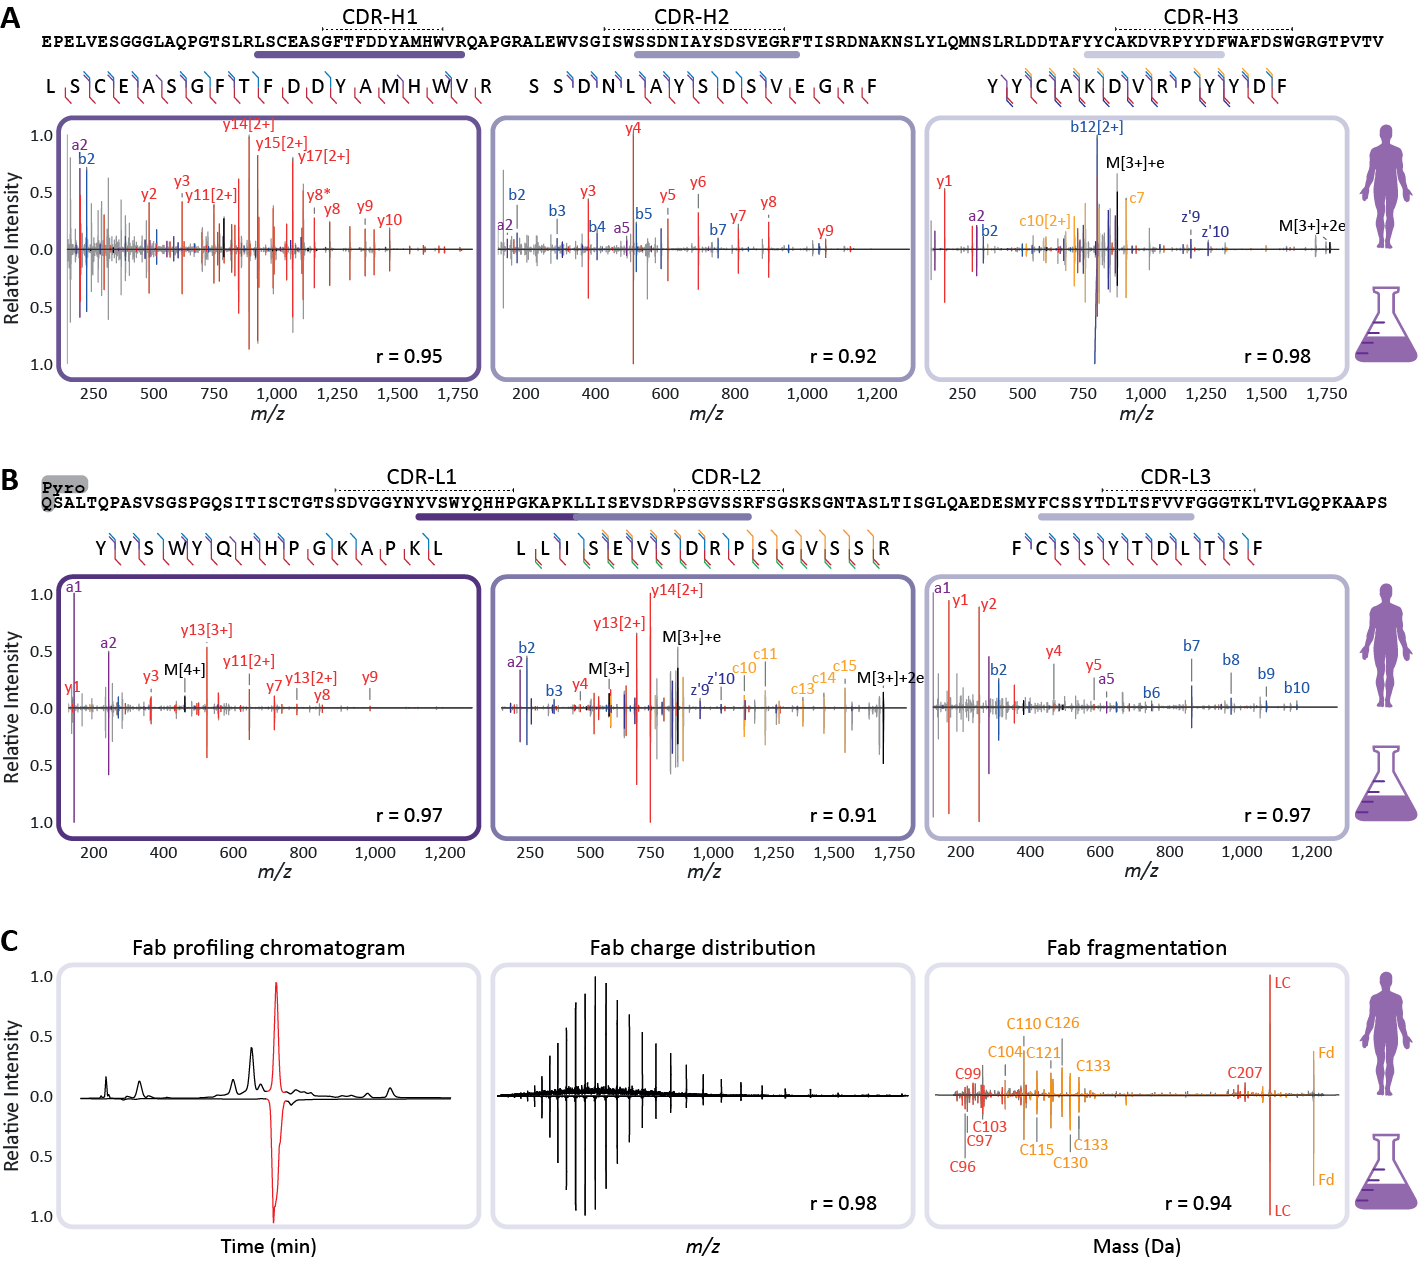
\includegraphics[]{Chapter.3/Figures/f5.png}
  \caption{
    \textbf{Comparison of sequencing data for clone \textsuperscript{24.4} 1 \textsubscript{47,359.4} of the donor F59, and the corresponding recombinant mAb validates the correctness of the \emph{de novo} sequencing approach.} ~~a) Peptide fragmentation spectra of CDR-spanning peptides from the HC of the dominant \textsuperscript{24.4} 1 \textsubscript{47,359.4} clone with, mirrored to each other, annotated spectra from the donor (top) and the recombinant IgG1 (bottom). ~~b) Peptide fragmentation spectra of CDR-spanning peptides from the LC of the dominant \textsuperscript{24.4} 1 \textsubscript{47,359.4} clone with, mirrored to each other, annotated spectra from the donor (top) and the recombinant IgG1 (bottom). Spectra in ~~a) and ~~b) are annotated with \emph{a}-ions in purple, \emph{b}-ions in blue, \emph{y}-ions in red, \emph{c}-ions in orange, and \emph{z}-ions in dark blue. Corresponding fragmentation maps are displayed above each spectral pair. ~~c) Comparison of the middle-down LC-MS/MS analysis of the \textsuperscript{24.4} 1 \textsubscript{47,359.4} clone and the recombinant IgG1. Shown are the base peak chromatograms (left panel), the charge-state distributions detected in MS1 of the Fab (middle panel), and the deconvoluted ETD fragmentation spectra for the donor (top) and recombinant (bottom) IgG (right panel). The Pearson correlation coefficients (r) calculated for all demonstrated spectral pairs in ~~a) , ~~b) , and ~~c) are indicated at the bottom of each spectrum.
  }
  \label{fig:fig3.5}
\end{figure*}


Such a direct comparison of spectral features was extended to the middle-down analysis, used for obtaining sequence tags of the intact Fab (\textbf{\autoref{fig:fig3.5}c}). The intact recombinant Fab displayed a nearly identical retention time profile when compared with the plasma clone \textsuperscript{24.4} 1 \textsubscript{47,359.4} Fab (\textbf{\autoref{fig:fig3.5}c}, left panel). Furthermore, both clone \textsuperscript{24.4} 1 \textsubscript{47,359.4} and the recombinant mAb emerged with nearly identical charge distributions (\textbf{\autoref{fig:fig3.5}c}, middle panel), whereby the slight differences in the distribution are likely due to the underlying background of co-eluting Fabs in the plasma-derived sample. Nevertheless, the masses detected for the two Fabs were identical, i.e., within a 20-ppm mass error. Moreover, when the intact Fabs were subjected to ETD, alike fragment masses and retention times for both the light chain and Fd were observed, comparing the recombinant mAb with the plasma-derived clone. Finally, the generated lower mass fragment ions used for sequence-tag generation were also very similar (\textbf{\autoref{fig:fig3.5}c}, right panel). Likewise, the in-solution reduction of the Fabs revealed that there were no mass differences between the donor clone and recombinant mAb (light chain and Fd mass within 10 ppm).
Based on all these data, we can conclusively state that the sequence of the plasma-derived clone \textsuperscript{24.4} 1 \textsubscript{47,359.4} is identical to that of the recombinant mAb, with practically identical data observed at every step of our integrative \emph{de novo} sequencing approach. This not only validates the accuracy of the IgG1 sequence that we obtained for clone \textsuperscript{24.4} 1 \textsubscript{47,359.4} but also reinforces that the methodology presented here can be used to derive the correct full sequences from individual clones even when they are in a background of other plasma (highly sequence-homologous) IgG1 clones. Although this whole analysis pipeline is still quite arduous, requiring manual validation throughout the process, we consider this proof of concept a major step forward and expect that further fine-tuning of the algorithms will enhance the throughput in the future.

\section{Discussion}
The human body can make billions of different antibodies, stemming from the versatile and complex recombination process, accompanied by additional somatic hypermutations, helping us to adapt to a life-long exposure to various pathogens. Here, we demonstrate that it is feasible to profile the IgG1 repertoire of individual donors qualitatively and quantitatively by LC-MS, following the capturing of IgGs from plasma and analyzing the generated IgG1 Fab fragments. From this technical advance, one of the key observations we make is that in all studied donors at all time points, only a limited number of IgG1 clones dominate an individual’s repertoire. In all donors, the 30 most abundant clones make up two-thirds of all detected circulating IgG1 molecules; in one donor just two clones contributed $\sim$50\% to the detected serum population of IgG1 molecules. The IgG1 clonal profiles are found to be unique for each donor. Within a donor, the profiles are highly similar across time, but they also adapt to physiological changes (e.g., sepsis). The mass-spectrometry-based approach requires only minute amounts of plasma ($\sim$10 μL) and does not involve labor-intensive enrichment protocols. We further show that specific IgG clones can be extracted from the plasma and analyzed in depth, ultimately leading to the mass-spectrometry-based \emph{de novo} sequencing of the whole Fab molecule. Therefore, one of the holy grails in proteomics, \emph{de novo} sequencing of antibodies directly extracted from plasma, seems to be within reach.
The ultimate mature sequence of \textsuperscript{24.4} 1 \textsubscript{47,359.4} clone we sequenced here revealed that around 13\% and 16\% of the amino acids of the V-regions of light and heavy chains were different when compared with the closest germline sequence match within the IMGT database. This number of mutations is higher than the reported average (7\%) for IgG1 heavy-chain variable regions, as determined from RNA sequences \cite{kitaura2017different}. This suggests that DNA/RNA templates of the IgG sequences can be helpful, but for obtaining the correct sequence of the circulating clone, analyzing sequences at the level of the proteins will be essential.
The ability to \emph{de novo} sequence the whole Fab molecule is the result of combining, iteratively, middle-down and bottom-up proteomics data. An alternative strategy employed is to combine bottom-up proteomics data with BCR sequences using RNA sequencing of one donor to generate a database to match this donor’s Ig bottom-up proteomics data against \cite{lee2016molecular-level}. Although also very powerful, a recent application of this approach highlighted further the relevance of antibody sequencing at the level of proteins, when it was shown that for the six potent anti-HIV1 antibodies found by antigen-specific single-B-cell sequencing, only three could also be detected in circulation as IgG protein products \cite{williams2017potent}. All these issues highlight the necessity of direct analysis of the serum Ig repertoire at the protein level, as we now demonstrated here to be feasible.
Longitudinal quantitative clonal profiling, as presented here, opens a myriad of future prospects, both fundamental and applied. It allows to advance our understanding of B cell biology and antibody dynamics. Historically, general observations have been made about antibody half-lives using a single dose of labeled antibodies \cite{morell1970metabolic} or by determining the restoration of normal IgG levels following high-dose administrations of intravenous IgG \cite{melamed2018pharmacokinetics}. Through the method presented here, we can monitor the longitudinal abundance of each single clone in the circulation and monitor how it responds to changes in the donor’s physiology. Given the approximately 20-day IgG antibody half-life, it is expected that in the time span studied here (10–63 days), a decay in the concentration of clones would be detected. Indeed, we do observe several diminishing clones as depicted in \textbf{\autoref{fig:fig3.2} and \autoref{fig:figs3.4}}. However, other patterns are also observed, indicative of continuous production of the clone, even over a time window of two months. This is in line with previous reports on the presence of and production of antibodies by long-lived plasma cells, both in mice and humans \cite{bernasconi2002maintenance, manz1997lifetime, slifka1998humoral}. In addition, persistence of autoreactivity has been reported before \cite{tebani2020integration}, as well as persistence of antibody clonotypes detected by CDR-H3 proteomics \cite{lee2019persistent}. From our data, we cannot derive information regarding (auto)reactivity, but the data do suggest that long-term stability is not exclusive to autoantibodies and is instead a common phenomenon.
In summary, the \emph{de novo} sequencing at the protein level of IgG clones circulating in plasma is shown here to be feasible. We demonstrate the synergistic power of combining iteratively peptide- and protein-centric-based sequencing, which is capable of not only identifying the distinct alleles from which a clone originates but also its entire mature sequence. The work presented here is still quite a laborious proof of concept. Our aim for the future is quantitative monitoring and mass-spectrometry-based sequencing of multiple serum immunoglobulins directly at the protein level, i.e., as they appear in circulation and function in the human immune response.

\subsection{Experimental model and subject details}

\subsubsection{Human subjects}
We obtained longitudinal plasma samples from the Molecular Diagnosis and Risk Stratification of Sepsis (MARS) biorepository (ClinicalTrials.gov identifier NCT01905033), for which subjects had been included in the mixed ICU of a tertiary teaching hospital in the Netherlands (University Medical Centre Utrecht, Utrecht) since January 2011. Donors were enrolled via an opt-out consent method approved by the institutional review board of the UMC Utrecht (IRB no. 10-1056C). Daily leftover EDTA plasma (obtained from blood drawn during routine care) was stored at -80 °C until use.
For the current study, we included eight patients with esophageal or gastroesophageal junction cancer who underwent an elective esophagectomy and gastric pull-through procedure and had subsequently developed an infectious complication (i.e., anastomotic leakage or pneumonia). These patients were all admitted to the Intensive Care Unit on two occasions. The first admission concerned routine observation after elective resection followed by an uncomplicated ICU stay of fewer than 2 days. All patients were subsequently readmitted to the ICU due to sepsis. For all episodes of sepsis, microbiological cultures were obtained either before or during ICU readmission, and clinical infection was adjudicated highly plausible according to pre-defined criteria \cite{klouwenberg2013interobserver}. Furthermore, all infectious episodes met SIRS criteria and had a Sequential Organ Failure Assessment (SOFA) score ≥ 2, thus fulfilling current Sepsis-3 definitions \cite{singer2016third}. All patients were ultimately discharged from ICU in a clinically stable condition. We analyzed plasma samples obtained at four well-defined time points: within 24 hours of surgery when no signs of sepsis were present (sample T1), on two consecutive days after onset of sepsis (samples T2 and T3), and upon ICU discharge following resolution of sepsis (sample T4). Patient characteristics are summarized in \textbf{Data \ref{tab:tabdummy3.2}}. All patients had been treated with neoadjuvant chemoradiotherapy prior to surgery. None of the patients received treatment with immunoglobulins or monoclonal antibodies either prior to or during ICU admission.
In addition, longitudinal EDTA plasma samples from two healthy Caucasian donors were purchased from Precision Med (Solana Beach, CA, US). The samples were part of the ‘Normal Control Collections’, protocol number 7005-8200. These donors were selected having similar characteristics as the sepsis donors regarding age and gender.

\subsection{Method details}

\subsubsection{Plasma IgG purification and Fab generation}
The IgG purification and generation of Fabs was adapted from an earlier published protocol \cite{bondt2014immunoglobulin}. The FcXL affinity matrix used in the workflow, which binds to the CH3 domain of the IgG constant region, has recently been shown not to provide a bias regarding analysis of the Fc glycosylation residing in the CH2 domain \cite{amezmartín2021serum}. Mobicol spin filters were assembled according to the manufacturer’s instructions and placed in 2 mL Eppendorf tubes. Then 20 μL FcXL affinity matrix slurry was added to the spin filter, followed by three washing steps with 150 μL PBS, in which the liquid was removed by centrifugation for 1 min at 1000 × g. Two additional washing steps with 150 μL were performed. After washing, the 2 mL tube was replaced by a 1.5 mL tube. The affinity matrix was resuspended in 150 μL PBS, and 10 μL plasma was added. Furthermore, 1 μL of a solution containing two known mAbs at 200 μg/mL each was added, corresponding to 20 μg/mL when calculated to the plasma concentration. The samples were then incubated, under shaking conditions for one hour at room temperature. After the incubation, the flow-through was collected, and the affinity matrix with bound IgGs was washed four times with 150 μL PBS. Finally, 50 μL PBS containing 100 U of the IgdE (FabALACTICA; Genovis AB, Lund, Sweden) protease was added before incubating on a thermal shaker at 37 °C for >16 hours. After the incubation, 10 μL of Ni-NTA beads were added to bind and remove the His-tagged protease, whereafter the samples were incubated for an additional 30 minutes. The flow through after centrifugation contained the Fab fragments generated from IgG1.

\subsubsection{Method optimization and validation using a mixture of recombinant mAbs}
In an array of experiments, we optimized and validated the robustness and accuracy of our IgG1 capturing approach, the generation of the Fab fragments and the analysis of the Fab LC-MS profiles. Therefore, we prepared a mixture of six IgG1 monoclonal antibodies, including the two spiked into every plasma sample subsequently analyzed. For the method optimization the 6 recombinant mAbs were added to the plasma of a single donor in different quantities: 4,000, 800, 200, 20, 2, or 0.5 ng per mAb. The mAbs used were trastuzumab (Roche, Penzberg, Germany), alemtuzumab (Genmab, Utrecht, The Netherlands), the Fab glycosylated cetuximab, rituximab, bevacizumab, and infliximab (Evidentic, Berlin, Germany). Fab sequences and theoretical masses of these mAbs, including the most abundant cetuximab glycoforms, are shown in \textbf{Data \ref{tab:tabdummy3.1}}. All these samples were injected once, except for the 200 ng sample which was injected three times to provide additional injection replicates.

\subsubsection{LC-MS(/MS)}
Reversed-phase liquid chromatography was performed by using a Thermo Scientific Vanquish Flex UHPLC instrument, equipped with a 1 mm x 150 mm MAbPac RP analytical column, directly coupled to an Orbitrap Fusion Lumos Tribrid (Thermo Scientific, San Jose, CA, USA) or Q Exactive HF-X mass spectrometer (Thermo Fisher Scientific, Bremen, Germany). The column preheater, as well as the analytical column chamber, were heated to 80 °C during chromatographic separation. Both samples, either containing intact Fabs or separate Fab chains, were separated over 62 min at a 150 μL/min flow rate. Gradient elution was achieved by using two mobile phases A (0.1\% HCOOH in Milli-Q) and B (0.1\% HCOOH in CH3CN) and ramping up B from 10 to 25\% over one minute, from 25 to 40\% over 55 min, and from 40 to 95\% over one minute. MS data were collected with the instrument operating in Intact Protein and Low Pressure mode. Spray voltage was set at 3.3 kV, capillary temperature 350 °C, probe heater temperature 100 °C, sheath gas flow 35, auxiliary gas flow 10, and source-induced dissociation was set at 15 V. The electrospray voltage was applied after 2 min to prevent the salts in the sample from entering the MS. Intact Fabs were recorded with a resolution setting of 7,500 (@ \emph{m/z} 200) in MS1, which allows for better detection of charge distributions of the large proteins (> 30 kDa) \cite{waterbeemd2018dissecting}. Separate Fab chains were analyzed with a resolution setting of 120,000 (@ \emph{m/z} 200) in MS1, which allows for more accurate mass detection of smaller proteins (< 30 kDa). MS1 scans were acquired in a range of 500-3,000 Th with the 250\% AGC target and a maximum injection time set to either 50 ms for the 7,500 resolution or 250 ms for the 120,000 resolution. In MS1, 2 μscans were recorded for the 7,500 resolution and 5 μscans for the 120,000 resolution per scan. Data-dependent mode was defined by the number of scans: single scan for intact Fabs and two scans for separate Fab chains. In both cases, MS/MS scans were acquired with a resolution of 120,000, a maximum injection time of 500 ms, a 1,000\% AGC target, and 5 μscans averaged and recorded per scan. The ions of interest were mass-selected by quadrupole in a 4 Th isolation window and accumulated to the AGC target prior to fragmentation. The electron-transfer dissociation (ETD) was performed using the following settings: 16 ms reaction time, a maximum injection time of 200 ms, and the AGC target of 1e6 for the ETD reagent. For the data-dependent MS/MS acquisition strategy, the intensity threshold was set to 2e5 of minimum precursor intensity. MS/MS scans were recorded in the range of \emph{m/z} = 350-5,000 Th using high mass range quadrupole isolation.

\subsubsection{Clonal profiling data analysis}
Masses were retrieved from the generated RAW files using BioPharmaFinder 3.2 (Thermo Scientific). Deconvolution was performed using the ReSpect algorithm between 5 and 57 min using 0.1 min sliding window with 50\% offset and a merge tolerance of 50 ppm, with noise rejection set at 95\%. The output mass range was set at 10,000 to 100,000 with a target mass of 48,000 and mass tolerance of 30 ppm. Charge states between 10 and 60 were included, and the Intact Protein peak model was selected. Further data analysis was performed using Python 3.8.10 (with libraries: Pandas 1.2.4 \cite{mckinney2010data}, Numpy 1.20.2 \cite{walt2011numpy}, Scipy 1.6.2 \cite{virtanen2020scipy}, Matplotlib 3.3.4 \cite{hunter2007matplotlib:} and Seaborn 0.11.1). Masses of the BioPharmaFinder identifications (components) were recalculated using an intensity weighted mean considering only the most intense peaks comprising 90\% of the total intensity. Furthermore, using the data of two spiked-in mAbs (trastuzumab and alemtuzumab) a mass correction was applied based on the difference between the calculated and observed mAb masses, and similarly, a retention time alignment was applied to minimize deviation between runs.
Components between 45,000 and 53,000 kDa with the most intense charge state above \emph{m/z} 1,000 and score ≥40 were considered Fab portions of IgG clones. The clones were matched between runs using average linkage (unweighted pair group method with arithmetic mean UPGMA) L∞ distance hierarchical clustering. Flat clusters were formed based on a cophenetic distance constraint derived from the mass and retention time tolerance. These tolerances were defined as three times the standard deviation of the mAb standards, which were 1.4 Da and 0.8 min, respectively. Clones within a flat cluster were considered identical between runs.

\subsubsection{Peptide-centric (bottom-up) \emph{de novo} sequencing}
Clones of interest were captured through fraction collection using the same chromatography setup used for LC-MS profiling. Samples were dried under vacuum and resuspended in a 50 mM ammonium bicarbonate buffer. To boost signal intensity, the fractions were pooled across the time points. Samples were equally split for digestion with four proteases.
For digestion with trypsin, chymotrypsin and thermolysin, a sodium deoxycholate (SDC) buffer was added to a total volume of 80 μL, 200 mM Tris pH 8.5, 10 mM tris(2-carboxyethyl)phosphine (TCEP), 2\% (w/v) SDC final concentration. For pepsin digestion, a urea buffer was added to a total volume of 80 μL, 2M Urea, 10 mM TCEP. Samples were denatured for 10 min at 95 °C followed by reduction for 20 min at 37 °C. Next, iodoacetic acid was added to a final concentration of 40 mM and incubated in the dark for 45 min at room temperature for alkylation of free cysteines. Then for trypsin, chymotrypsin and thermolysin 50 mM ammonium bicarbonate buffer was added to a total volume of 100 μL. For pepsin 1 M HCl was added to a final concentration of 0.04 M. 0.1 μg of each protease was added and incubated for 4 hours at 37 °C. After digestion 2 μL HCOOH was added to precipitate the SDC. SDC was removed by centrifugation for 20 min at max speed (20,817 × ~~g) after which the supernatant was moved to a new tube.
Samples were desalted by Oasis HLB (Waters Corporation, Millford, MA, USA) following a 5-step protocol. 1) Sorbent was wetted using 2x 200 μL CH3CN, 2) followed by equilibration with 2x 200 μL water/10\% HCOOH. 3) The sample was loaded and 4) washed with 2x 200 μL water/10\% HCOOH. 5) Finally, the sample was eluted using 2x 50 μL water/50\% CH3CN /10\% HCOOH and dried down by vacuum centrifuge. Prior to MS analysis samples were reconstituted in 2\% HCOOH.

\paragraph{LC-MS/MS}
Data acquisition was performed on the Orbitrap Fusion Tribrid Mass Spectrometer (Thermo Scientific, San Jose, CA, USA) coupled to UHPLC 1290 system (Agilent Technologies, Santa Clara, CA, USA). Peptides were trapped (Dr. Maisch Reprosil C18, 3 μm, 2 cm × 100 μm) prior to separation (Agilent Poroshell EC-C18, 2.7 μm, 500 mm × 75 μm). Trapping was performed for 10 min in solvent A (0.1\% HCOOH in Milli-Q), and the gradient was as follows: 0 – 13\% solvent B (0.1\% HCOOH in 80\% CH3CN) over 5 min, 13 – 44\% solvent B over 65 min, 44 – 100\% solvent B over 4 min, and 100\% B for 4 min (flow was split to achieve the final flowrate of approximately 200 nL/min). Mass spectrometry data was collected in a data-dependent fashion with survey scans ranging from 350-2,000 Th (resolution of 60,000 @ \emph{m/z} 200), and up to 3 sec for precursor selection and fragmentation with either stepped higher-energy collisional dissociation (HCD) set to [25\%, 35\%, 50\%] or electron transfer dissociation (ETD), used with charge-normalized settings and supplemental activation of 27\%. The MS2 spectra were recorded at a resolution of 30,000 (@ \emph{m/z} 200). The AGC targets for both MS and MS2 scans were set to standard within a maximum injection time of 50 and 250 ms, respectively.

\paragraph{Data analysis}
Raw LC-MS/MS data were processed using PEAKS X software (Bioinformatics Solutions Inc., Waterloo, ON, Canada) for \emph{de novo} sequencing of peptides. The following parameters were used for \emph{de novo} sequencing: parent mass error tolerance – 12 ppm, fragment mass error tolerance – 0.02 Da, max number of variable PTMs per peptide – 3. Fixed modifications: Carboxymethyl; variable modifications: Oxidation (HW), Oxidation (M), Pyro-glu from E, Pyro-glu from Q, Carboxymethyl (KW, X@N-term), and Carbamylation. Resulting \emph{de novo} peptide tables were exported as.csv files and used for filtering of the IMGT database and determination of the mature \textsuperscript{24.4} 1 \textsubscript{47359.4} clone sequences.

\subsubsection{Protein-centric (middle-down) \emph{de novo} sequencing}
Fab samples were prepared without treatment as well as under denaturing and reducing conditions for analysis of intact Fab and separate Fab chains, respectively. The latter were denatured and reduced in 10 mM TCEP at 60 °C for 30 min prior to LC-MS/MS analysis. Approximately 2-5 μg of each sample was injected for a single middle-down LC-MS(/MS) experiment using the parameters described above.

\paragraph{Data analysis}
Full middle-down MS spectra were deconvoluted with either Xtract \cite{zabrouskov2005new} or ReSpect (Thermo Fisher Scientific, Bremen, Germany) for isotopically-resolved (separate Fab chains) or unresolved (intact Fabs) data, respectively. Middle-down LC-MS/MS data were charge-deconvoluted and deisotoped into singly-charged mass spectra using the ‘Parallel Xtract’ node and converted to mascot generic format (mgf) files in Thermo Proteome Discoverer (version 2.3.0.523; Thermo Fisher Scientific, Bremen, Germany). Deconvolution parameters were set as follows: ReSpect: precursor \emph{m/z} tolerance – 0.2 Th; relative abundance threshold – 0 \%; precursor mass range from 3 to 100 kDa; precursor mass tolerance of 30 ppm; charge states between 3 and 100. Xtract: signal/noise threshold of 3; \emph{m/z} range – 500-3,000 Th.
For the analysis of the final mature Fab chains of the most abundant clone in the plasma of patient F59, we used an integrative approach that utilizes bottom-up and middle-down data and the international ImMunoGeneTics information system (IMGT) database (\textbf{\autoref{fig:fig3.3}b}). First, the replicate middle-down MS/MS spectra were grouped per deconvoluted mass feature in the LC-MS-only runs by using a 3 Da mass window and a 3 min retention time window. The resulting grouped spectra were merged into a single spectrum, whereby peaks’ intensities were combined when they coincided within a 2 ppm window. The identity of the constant domain (C-) gene was determined by matching the fragments in these combined spectra to a database of all functional, open reading frame, and in-frame pseudogene alleles for C-genes retrieved from IMGT/Gene-DB \cite{lefranc1999imgt}. Next, bottom-up LC-MS/MS spectra of the fractionated \textsuperscript{24.4} 1 \textsubscript{47359.4} clone were screened against a database of all functional, open reading frame, and in-frame pseudogene alleles for the variable domain (V-) genes retrieved from the IMGT/Gene-DB \cite{lefranc1999imgt}, using local Smith-Waterman alignment with the BLOSUM62 matrix in which the common \emph{de novo} sequencing errors I/L, Q/E and N/D were modified to neutral substitutions \cite{smith1981identification}. From any gene regions with confident peptide matches (FDR < 1\%), we then took the FR1, 2 and 3 regions and subjected them to an in-house scoring algorithm to score their agreement with our middle-down data (\textbf{\autoref{fig:figs3.5}}). In short: the algorithm searches for peak patterns that would occur as a result of fragmentation of the provided sequence regions, disregarding preceding and succeeding parts of the initial sequence. Ranking the gene regions by a resulting composite score enabled us to select top-scoring templates as a starting point for our sequencing efforts as well as discard low-scoring regions from further analyses. The remaining gene regions were then used to in silico generate a database of germline light and heavy chains.
Then, using a custom implementation of the DirecTag algorithm \cite{tabb2008directag:}, all possible sequence tags were detected and annotated in the combined middle-down spectra. These sequence tags were used to search the filtered germline light and heavy IgG chains. For the best scoring germline sequences, consistent sequence tags with a length of more than 4 amino acids were searched against \emph{de novo} predicted peptides originating from the bottom-up peptide-centric MS data. In an iterative manner, the matching peptides were used to modify the best scoring selected germline sequences until the mass of the final sequence matched the precursor masses determined by middle-down MS (\textbf{\autoref{fig:figs3.8} and \autoref{fig:figs3.9}}). In more detail, the gaps between the consecutive sequence tags extracted from the middle-down MS data were first filled with amino acids from the best matching germline sequence. Then, the filled gaps were compared to the highest scoring peptides retrieved from the bottom-up MS data, aligned to the region of interest using Clustal Omega algorithm. When aligned peptides showed discrepancies from the germline sequence the amino acid residues in the gaps were altered and the theoretical mass of the gap was compared to the experimental mass, defined by the mass difference between consecutive sequence tags. Finally, the modified sequences were rescored by spectral alignment, sequence-tag detection, and a bottom-up database search, providing the final mature Fab sequences. The final predicted sequences – and more specifically the identified mutations when compared to the most closely related gene regions – were additionally compared to the frequency of amino acid occurrence at their specific positions (as numbered by IMGT) in both the AbYsis database \cite{swindells2017abysis:} and the recombined full IMGT database \cite{lefranc1999imgt}. This screening yielded an estimate of how likely the mutations were to occur. While some of the predictions are rather rare, none of them are impossible as reported by AbYsis (\textbf{Data \ref{tab:tabdummy3.5}}).

\subsection{Quantification and statistical analysis}
For quantification of LC-MS profiling data, the intensity values of the two mAb standards (trastuzumab and alemtuzumab) were averaged in each run and set to 20 μg/mL. The intensity values of all other detected Fabs were normalized to these values in order to determine the concentration of each individual clone. For the quantification of mAbs in the validation experiment, a slightly different normalization was used. The intensity values of the detected mAbs in all runs were normalized to the intensity values of trastuzumab and alemtuzumab as measured in the first 200 ng replicate.
Statistical values in figures depicted as lower-case letter r indicate Pearson correlation coefficients. Distances between samples as shown in \textbf{\autoref{fig:fig3.2}b} were determined by distance correlation. Linear regression for validation of quantification \textbf{\autoref{fig:figs3.1}b} was determined by ordinary least squares regression with the coefficient of determination given as uncentered R\textsuperscript{2}. The error-bars in the figure represent the standard error of the mean (SEM).

\section{Acknowledgments}
This research received funding through the Netherlands Organization for Scientific Research (NWO) through the ENPPS.LIFT.019.001 project (A.J.R.H. and J.F.G.), the NACTAR project 16442 (A.J.R.H. and M.A.d.B.), Gravitation Subgrant 00022 from the Institute for Chemical Immunology (A.B., D.M.H.v.R., W.P., D.S., and J.S.), and the Spinoza award SPI.2017.028 to A.J.R.H. This project received additional funding from the European Union’s Horizon 2020 research and innovation program under the grant agreement 686547 (EPIC-XS) for A.J.R.H. We kindly acknowledge the teams of Janine Schuurman, Frank Beurskens, and Boris Bleijlevens (Genmab, Utrecht, NL) for continuous support over the years, stimulating discussions, financial co-support for A.B. and S.T., and the generation of the recombinant clone based on the sequence of the plasma clone \textsuperscript{24.4} 1 \textsubscript{47,359.4}. We thank Dietmar Reusch and Markus Haberger (Roche, Penzberg) for the kind donation of trastuzumab.

\subsection{Author contributions}
A.J.R.H. conceived the idea for this study. A.B., S.T., and A.J.R.H. designed the research, planned the experiments, and supervised the project. A.B., M.H., M.A.d.B., and D.M.H.v.R. performed the IgG capture from serum and subsequent generation of Fabs, subsequently analyzed by intact LC-MS. M.H. developed the repertoire profiling bioinformatics workflow. S.T. performed the middle-down MS/MS analysis of the clones and in collaboration with S.C.d.G generated the bioinformatics workflow to analyze the data. W.P., M.H., D.S., and J.S. performed all bottom-up proteomics experiments and subsequent data analysis. S.T. and S.C.d.G performed the de novo sequencing through the  iterative integration of middle-down and bottom-up proteomics data. J.-F.G. contributed to study design and data analysis. M.V., M.J.M.B., and O.L.C. provided the MARS cohort samples and selected the patient population used in this study. A.B., M.H., S.T., and A.J.R.H. wrote the original draft, which was read, improved, and approved by all co-authors.

\subsection{Declaration of interests}
The authors declare no competing interests.
\clearpage
\begin{subappendices}

  \section{Supplementary material}
  \beginsupplement
  Supplementary Table 1-5 and Supplementary Data 1-3 can be found online at:\\
  \emph{https://doi.org/10.1016/j.cels.2021.08.008}\\

  \vspace{24cm}

  \refstepcounter{table}
  \label{data:datadummy3.1}
  \refstepcounter{table}
  \label{data:datadummy3.2}
  \refstepcounter{table}
  \label{data:datadummy3.3}
  \addtocounter{table}{-3}
  \refstepcounter{table}
  \label{tab:tabdummy3.1}
  \refstepcounter{table}
  \label{tab:tabdummy3.2}
  \refstepcounter{table}
  \label{tab:tabdummy3.3}
  \refstepcounter{table}
  \label{tab:tabdummy3.4}
  \refstepcounter{table}
  \label{tab:tabdummy3.5}
  \addtocounter{table}{-6}

  \begin{figure*}[!h]
    \center
    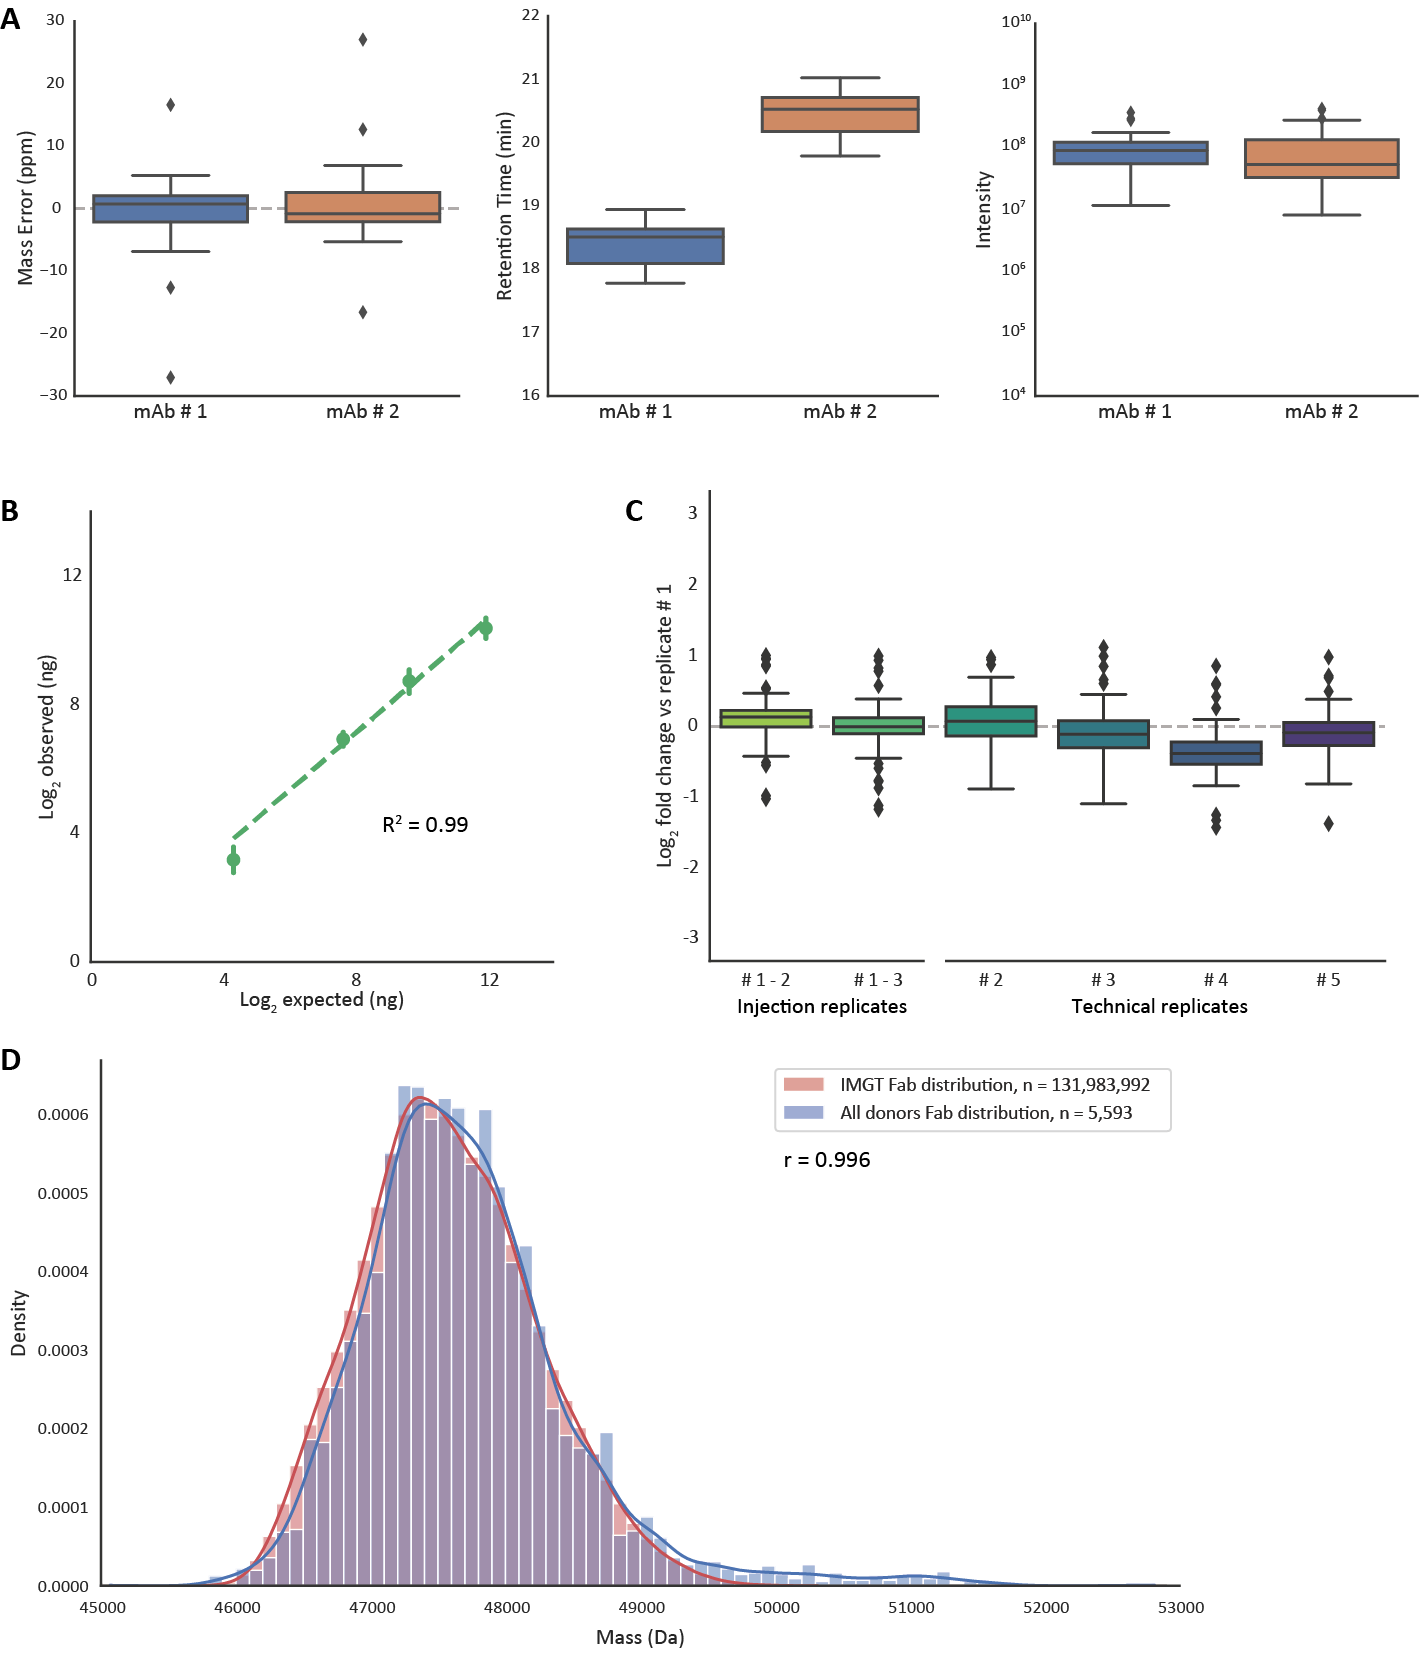
\includegraphics[]{Chapter.3/Figures/fs1.png}
    \captionsetup{singlelinecheck = false, format= hang}
    \caption{
      Figure legend on next page.
    }
    \label{fig:figs3.1}
  \end{figure*}
  \addtocounter{figure}{-1}
  \begin{figure*}[t!]
    \caption{
      \textbf{Performance evaluation of plasma Fab profiling approach using various experimental controls.} ~~a) Accuracy
      and precision in mass, retention time and abundance of spiked-in monoclonal antibody controls. The boxplots show aggregated data from the mAb controls over all plasma measurements. The box indicates median and inter quartile ranges (IQRs), and the whiskers span 1.5 times the IQR. Values outside this range (fliers) are marked with diamonds. From left to right, the panels show observed mass error of these mAbs, observed retention time, and detected intensity. ~~b) Linearity of detection. For these experiments six monoclonal antibodies (Trastuzumab, Cetuximab, Rituximab, Campath, Bevacizumab and Infliximab) were added at 20, 200, 800 and 4000 ng in a plasma background. The detected response of all of these mAbs was compared to the expected response visualized as scatterplot. The error bars depict the standard error, and the dotted line shows an ordinary least squares (OLS) linear regression accompanied by a R\textsuperscript{2}. ~~c) Reproducibility of quantitation. The reproducibility of the top 100 most intense clones in a plasma were measured over several replicates and visualized as boxplots. The values are shown as fold change of the concentration compared to the first replicate measurement. The first two boxplots depict injection replicates, i.e. replicates from multiple injections of the same sample. The other boxplots show technical replicates, which constitute the entire sample preparation procedure starting from the plasma. The boxes are constructed using the same method as the boxplots in panel ~~a) . ~~d) Distributions of detected Fab masses compared to the expected mass distribution. Kernel density estimation of all Fabs detected in all sepsis donors, at all analyzed time points, compared against an in silico generated distribution of Fabs from the IMGT database. The number of Fabs used to generate each distribution is shown in the Figure legend. Both distribution histograms use a bin size of 100 Da. The Pearson correlation coefficient (r) was calculated between both kernel density estimations.
    }
    \vspace{24cm}
  \end{figure*}

  \begin{figure*}[!p]
    \center
    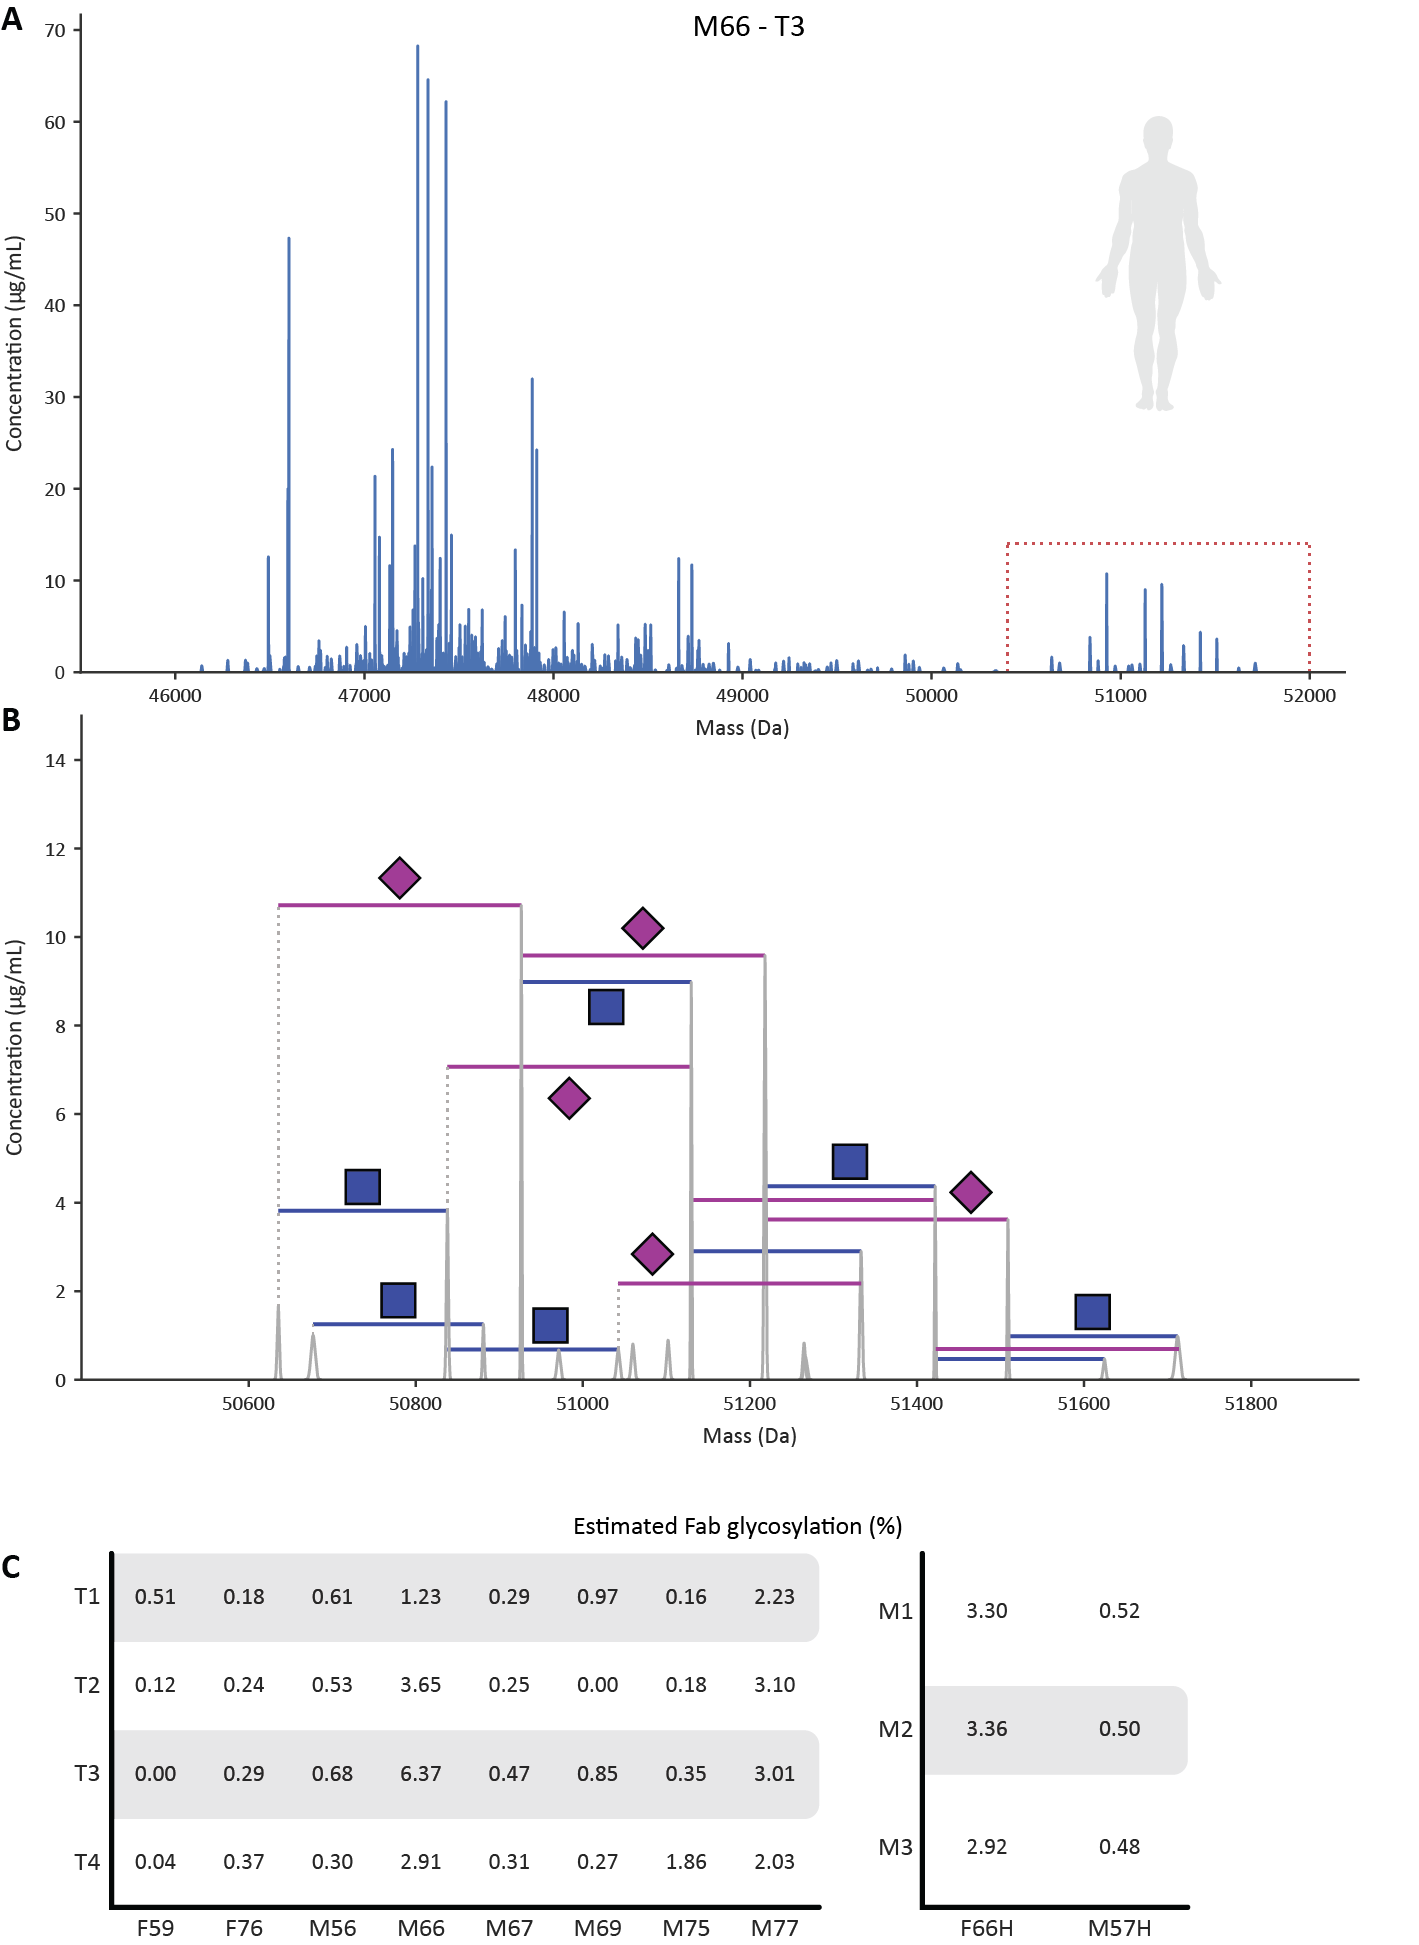
\includegraphics[]{Chapter.3/Figures/fs2.png}
    \captionsetup{singlelinecheck = false, format= hang}
    \caption{
      Figure legend on next page.
    }
    \label{fig:figs3.2}
  \end{figure*}
  \addtocounter{figure}{-1}
  \begin{figure*}[pt!]
    \caption{
      \textbf{Extent of Fab glycosylation in the plasma repertoire} ~~a) Fab mass profile of donor M66, taken from the plasma sample at time point 3. The mass range between 50,400 Da and 52,000 Da is boxed in red and shown magnified in panel ~~b) . ~~b) Zoomed-in mass profile with annotation of glycan-related masses. Monosaccharides mass differences between peaks are annotated as follows: blue square = GlcNAc (203 Da), magenta diamond = sialic acid (291 Da). For annotation of the glycosylation a mass tolerance of 1 Da and a retention time tolerance of 0.6 min was used. ~~c) Estimated percentages of plasma Fab molecules being glycosylated in all samples measured. For this, Fab clones with a mass >49,500 Da were assumed to carry one or more Fab glycans. This value was chosen because the in silico Fab distribution generated from the IMGT database (shown in \textbf{\autoref{fig:figs3.1}d}) extends up to 49,500 Da, the majority of Fabs has a mass between 47,000 and 48,000, and the average literature described Fab glycan has a mass of approximately 2,300 Da. The validity of this assumption is illustrated for M66 – T3 in panels ~~a) with the glycosylated Fabs being in mass quite separated from the other clones. The percentage of plasma Fab molecules being glycosylated was calculated by taking the sum of Fab concentrations above 49,500 Da and dividing these by the total detected concentration in each sample. On the left in ~~c) are shown the \% Fab glycosylation in the plasmas of the septic patients, on the right the \% observed in two healthy donors. In general, we observe that the \% Fab glycosylation is < 1\%, although in some donors it is substantially higher, i.e. M66, M77 and F66H.
    }
    \vspace{24cm}
  \end{figure*}
  \begin{figure*}[!hbt]
    \center
    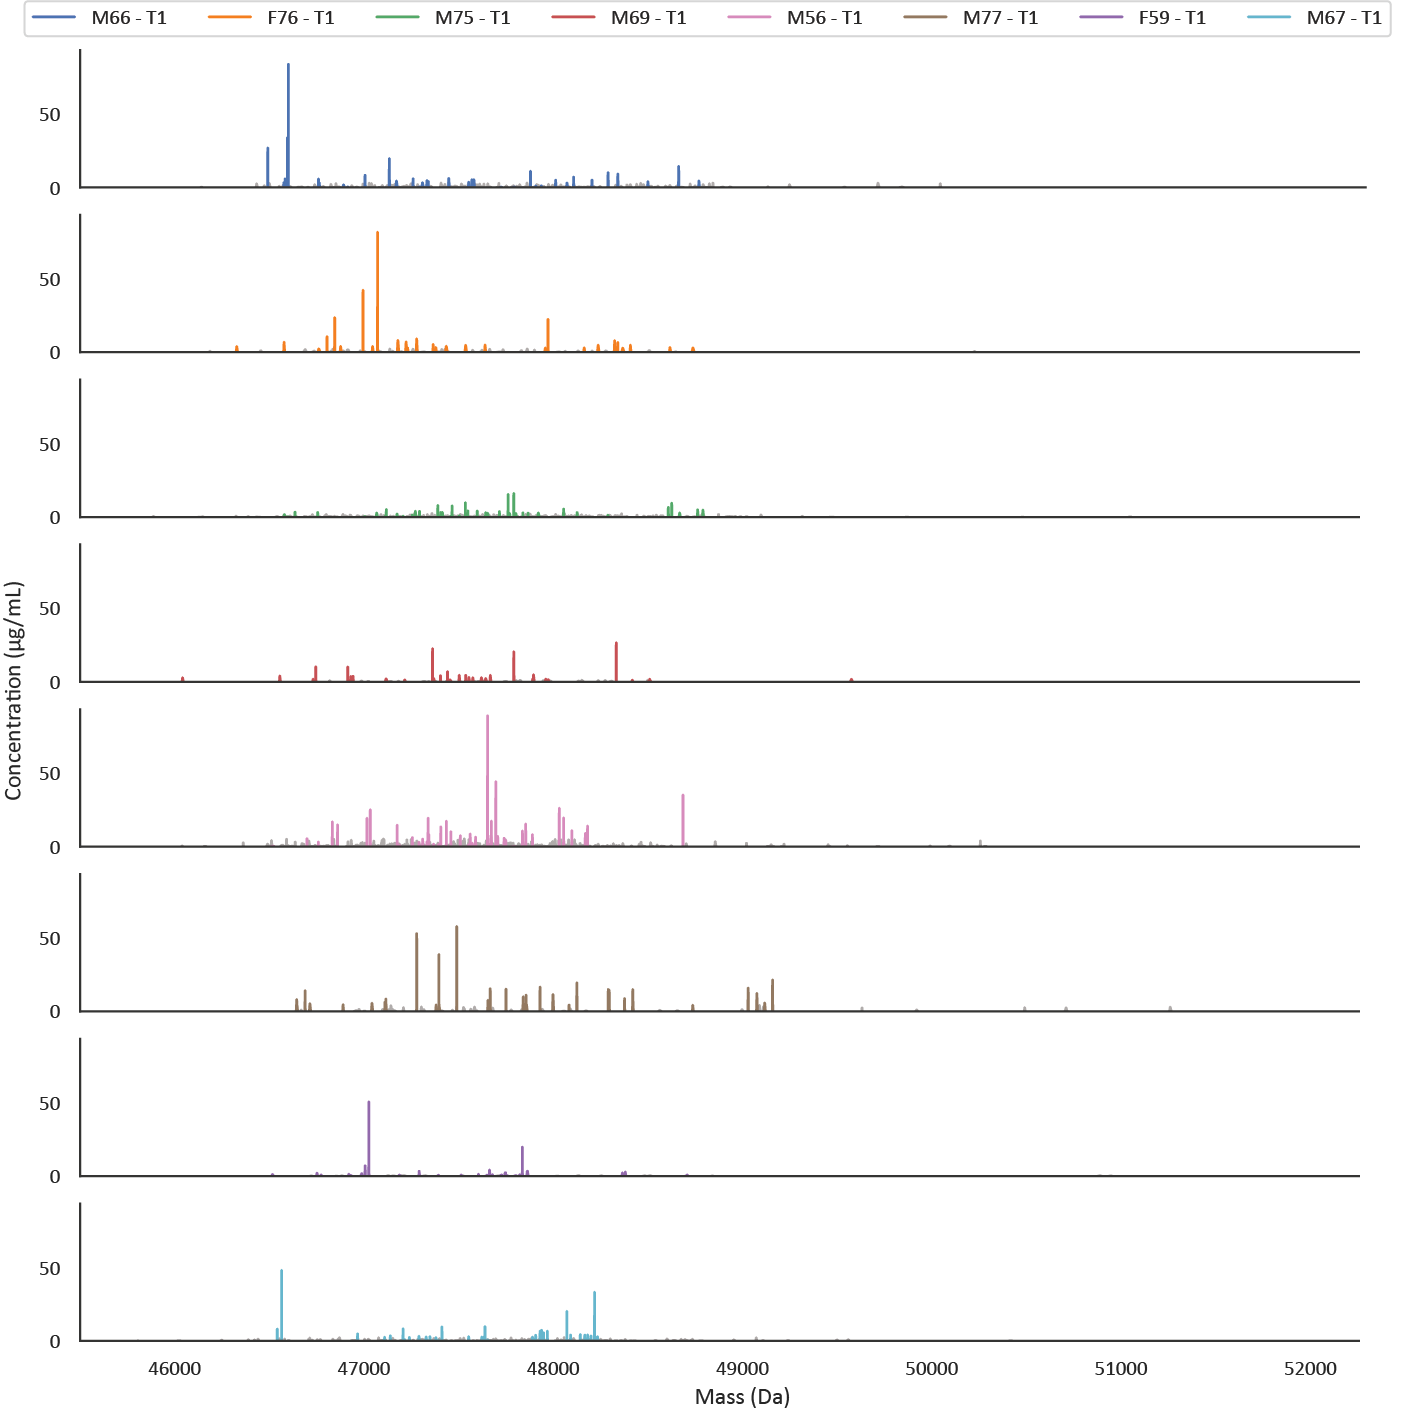
\includegraphics[]{Chapter.3/Figures/fs3.png}
    \caption{
      \textbf{Fab mass profiles are simple and uniquely individual.} The by LC-MS obtained Fab mass profiles are shown for plasma taken from each patient at time point 1 (post-operative). The Fab mass profiles are plotted along the full mass range. In each profile the top 30 most intense clones are colored, with a separate color for each donor. The remaining clones are shown in grey. The concentrations were determined from the LC-MS intensities, normalized against two spiked in recombinant mAbs.
    }
    \label{fig:figs3.3}
  \end{figure*}

  \vspace{1cm}

  \begin{figure*}[!p]
    \center
    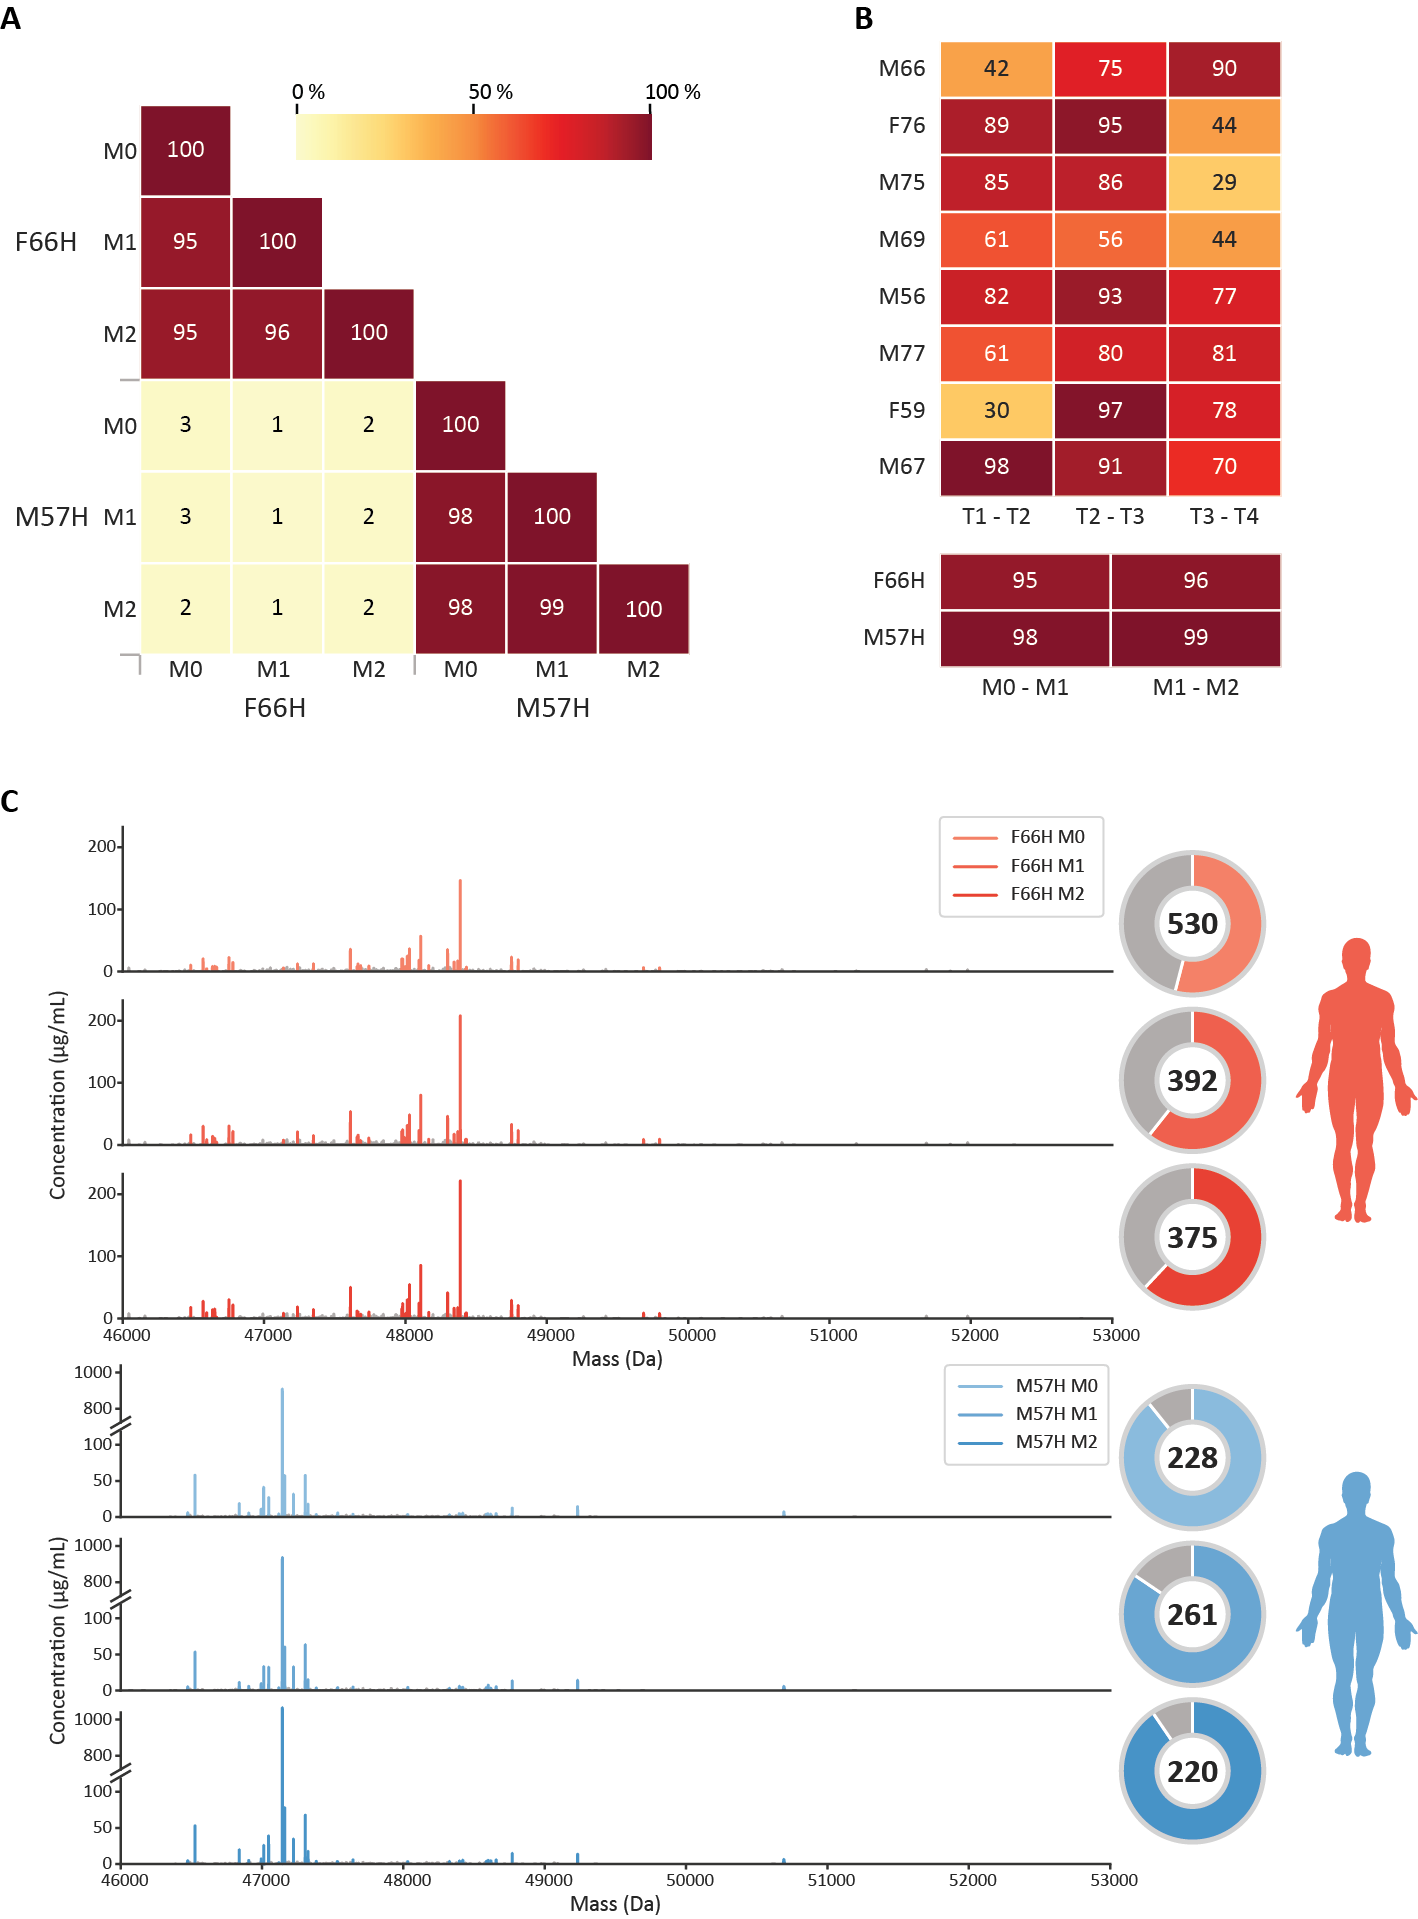
\includegraphics[]{Chapter.3/Figures/fs4.png}
    \captionsetup{singlelinecheck = false, format= hang}
    \caption{
      Figure legend on next page.
    }
    \label{fig:figs3.4}
  \end{figure*}
  \addtocounter{figure}{-1}
  \begin{figure*}[pht!]
    \caption{
      \textbf{Longitudinal plasma Fab profiles obtained for two healthy donors.} ~~a) Heatmap of healthy donors F66H and M57H constructed using the same method as used in \textbf{\autoref{fig:fig3.2}a}. Time points are marked M0, 1, and 2, representing month 0, month 1 and month 2, to clearly distinguish these from the sepsis donor time points. Inside each cell of the heatmap a percentage value shows the degree of overlap between samples, which is also represented by the color bar. ~~b) Heatmap showing the Fab overlap in consecutive time points of all healthy and sepsis affected donors, showing only the degree of overlap for consecutive time points within each donor. The colors match those of the color bar from panel A. ~~c) Mass profiles of healthy donors with donut charts. For each mass profile the top 30 most intense clones are colored, and the remaining clones are colored grey. In the donut charts the colored slice displays the distribution of the top 30 most intense clones compared to the other clones. The value inside the donut shows the total number of detected clones.
    }
  \end{figure*}

  \vspace{1cm}
  \begin{figure*}[!hbt]
    \center
    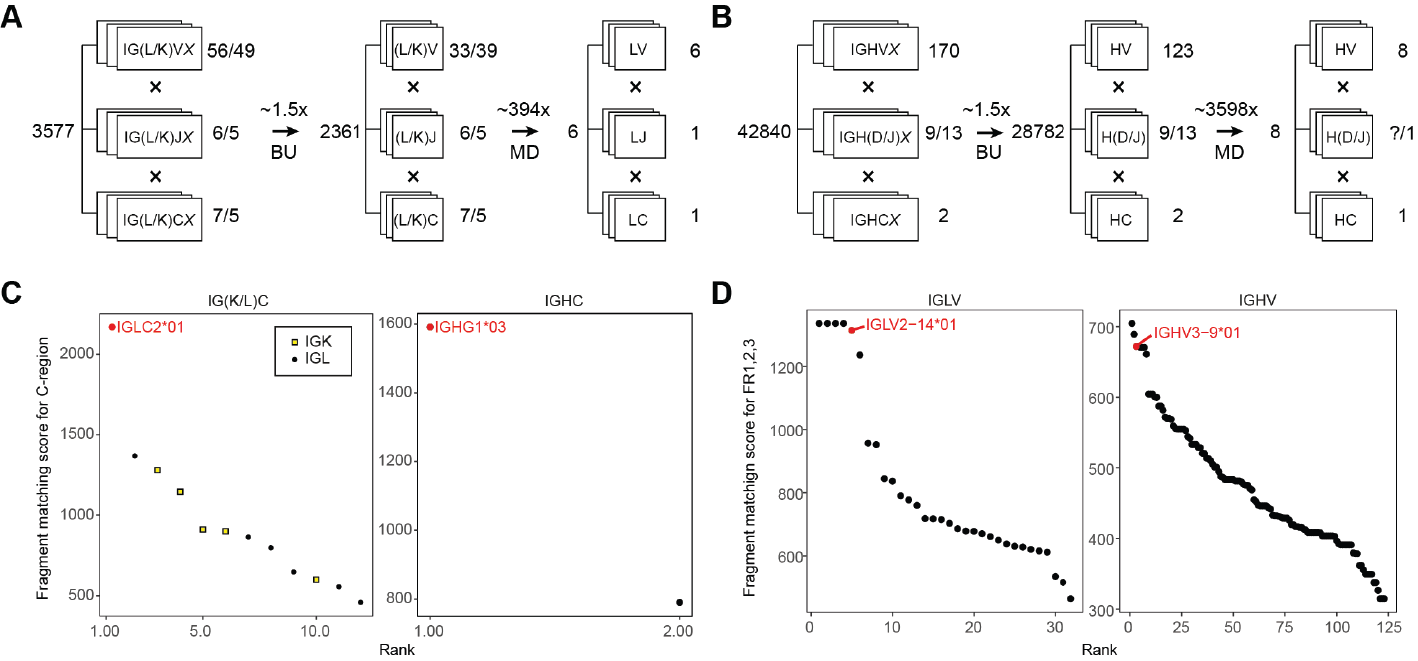
\includegraphics[]{Chapter.3/Figures/fs5.png}
    \caption{
      \textbf{Template matching of the obtained sequencing data for the Fab clone \textsuperscript{24.4} 1 \textsubscript{47359.4} versus the IMGT database.} The filtering of IMGT database and scoring of the germline IGXV and IGXC-alleles was performed by using iteratively bottom-up (BU) and middle-down (MD) proteomics data. ~~a) Filtering of germline IGL and IGK alleles with BU and MD mass spectrometry (MS) reduces the number of possible germline light chain sequences from 3,577 to 6 candidate sequences ($\sim$600-fold reduction). ~~b) Filtering of germline IGH alleles with BU MS and MD MS reduces the number of possible germline heavy chain sequences from 42,840 to 8 candidate sequences ($\sim$5,000-fold reduction). ~~c) Fragment matching scores for the germline C-gene alleles of the light (left) and heavy (right) chain of the Fab clone \textsuperscript{24.4} 1 \textsubscript{47359.4} using the middle-down MS data. ~~d) Fragment matching scores for the Framework Regions 1, 2, and 3 of the germline V-gene alleles of light (left) and heavy (right) chains of IgG1 determined by using the middle-down MS data.
    }
    \label{fig:figs3.5}
  \end{figure*}

  \vspace{1cm}

  \begin{figure*}[!ht]
    \center
    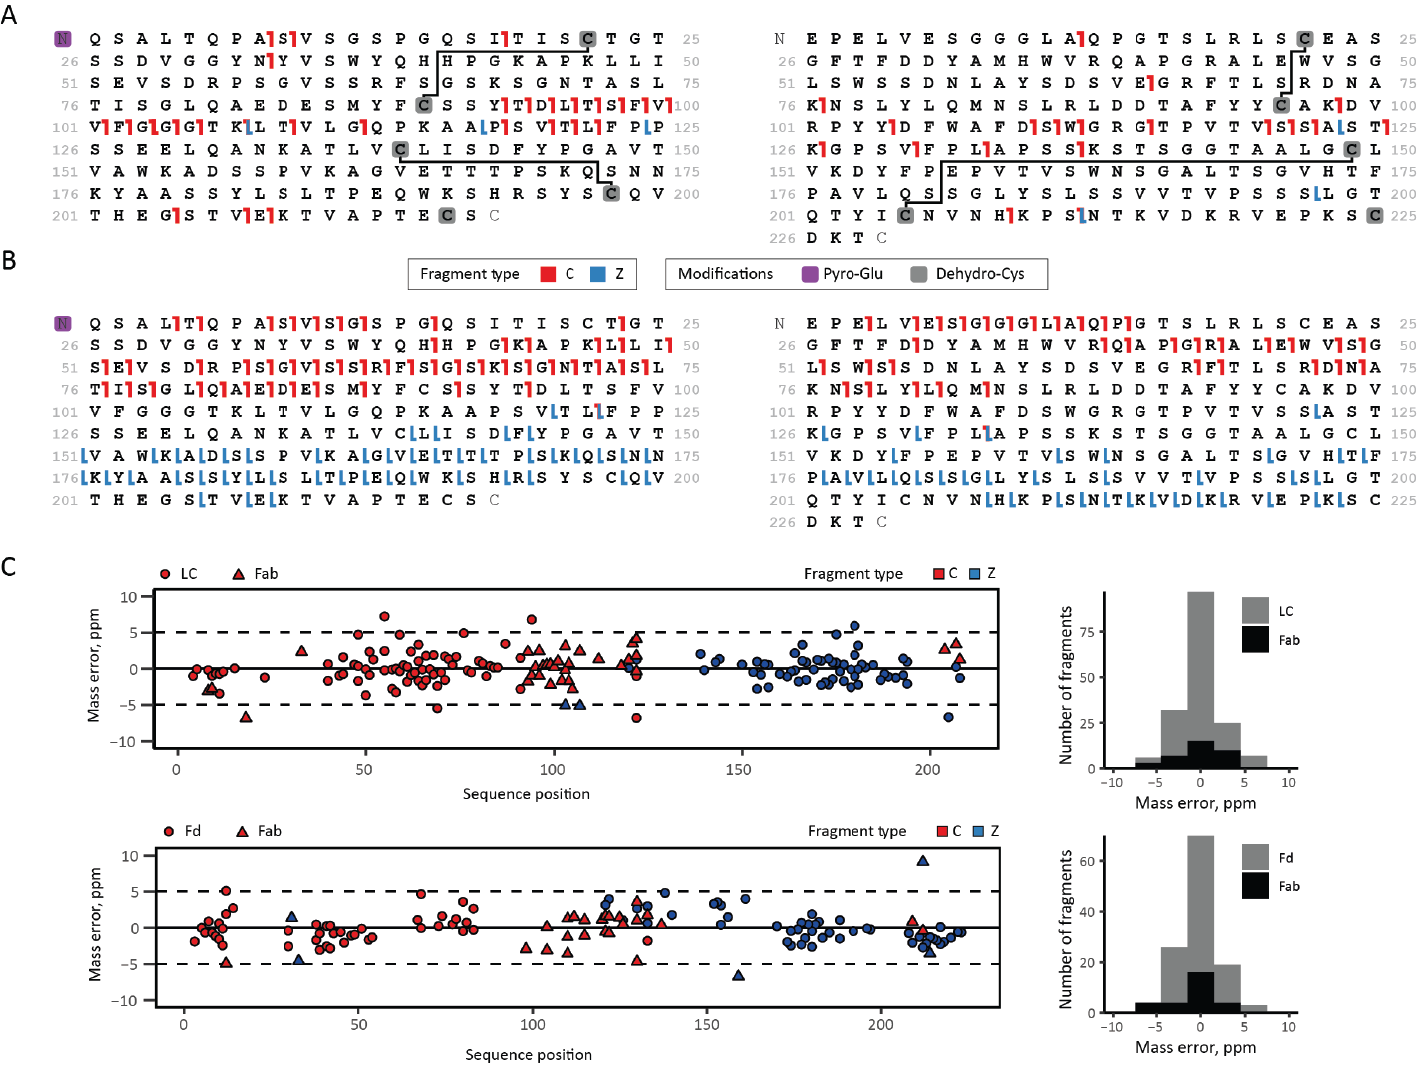
\includegraphics[]{Chapter.3/Figures/fs6.png}
    \caption{
      \textbf{Middle-down ETD analysis and sequence annotation of the light chain and the N-terminal portion of the
        heavy chain from clone \textsuperscript{24.4} 1 \textsubscript{47359.4} from donor F59.} ~~a) Fragmentation maps of the light chain (left) and Fd (right) when subjected to ETD within the intact Fab molecule. ~~b) Fragmentation maps of the light chain (left) and Fd (right) when subjected to ETD after reduction and denaturation of the precursor Fab. ~~c) Mass errors and their distribution of the light chain fragments observed in ETD of Fab and the light chain alone, and mass errors and distribution thereof for Fd fragments detected in ETD of Fab and Fd alone.
    }
    \label{fig:figs3.6}
  \end{figure*}

  \vspace{1cm}

  \begin{figure*}[!ht]
    \center
    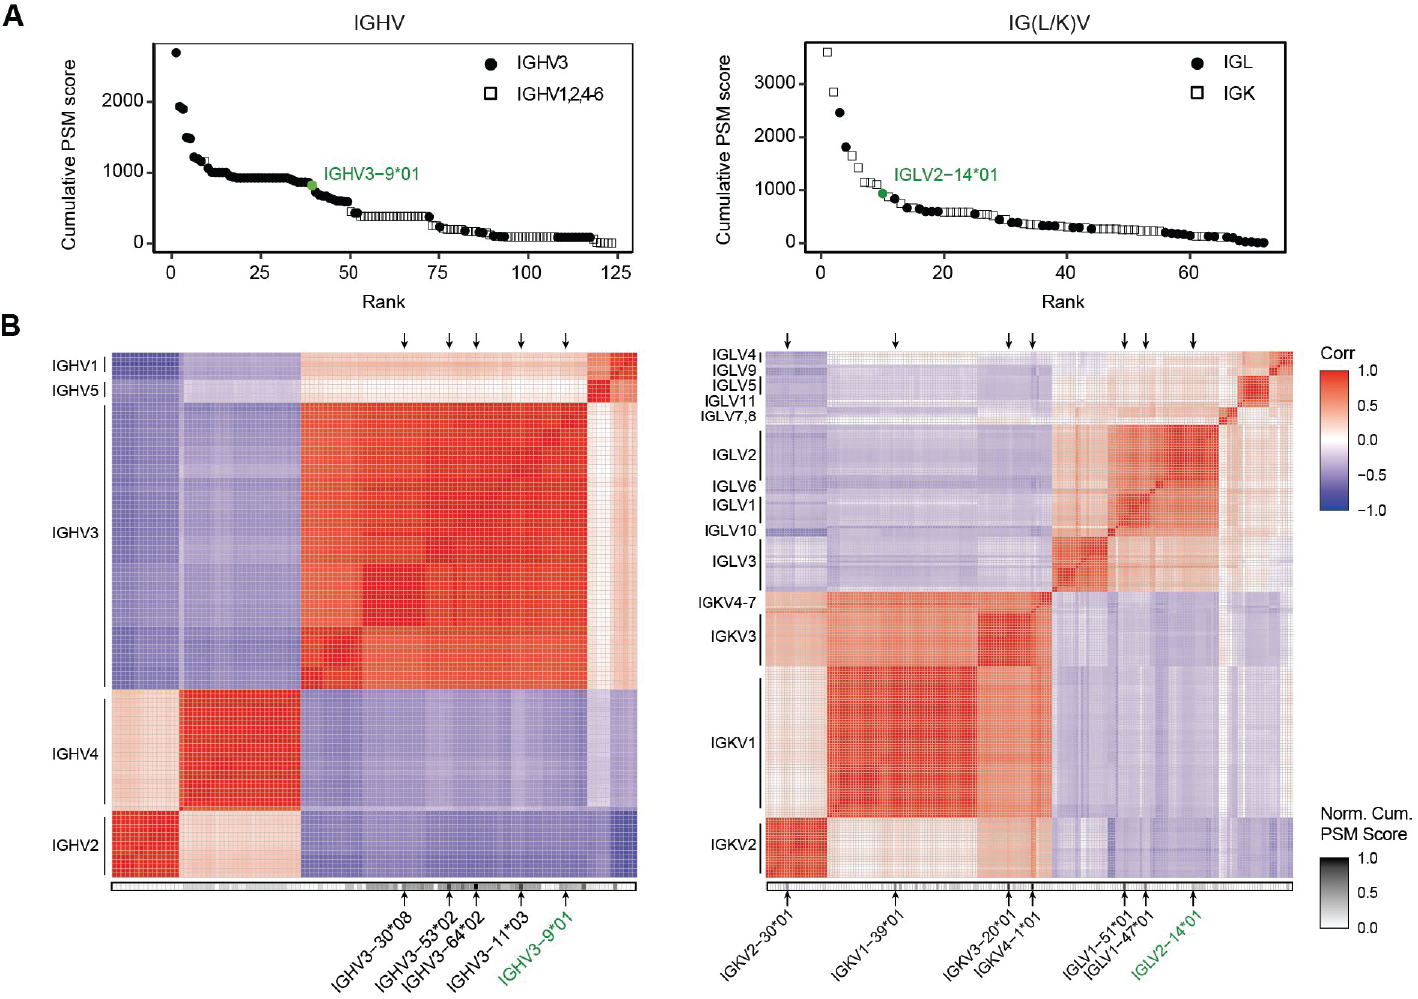
\includegraphics[]{Chapter.3/Figures/fs7.png}
    \caption{
      \textbf{Large homologous families of Ig V-gene alleles (e.g. IGHV3) are observed among the top-scoring identifications as extracted from the bottom-up proteomics data.} ~~a) Cumulative PSM scores determined for the germline V-gene alleles of the Fab heavy (left) and light chains (right). On the left, alleles from the largest IGHV3 family are displayed as filled circles; alleles of other IGHV families are shown as empty squares. On the right, alleles from larger and more homologous IGKV families are shown as empty squares, while filled circles display alleles of IGLV families. Germline V-gene sequences were downloaded from IMGT. ~~b) Correlation matrix displaying sequence similarity among all germline V-gene sequences of the Fab heavy (left) and light (right) chain. Normalized cumulative PSM scores are shown below the correlation maps. Some of the top-scoring V-gene sequences are indicated with black arrows. The V-genes ultimately determined for clone \textsuperscript{24.4} 1 \textsubscript{47359.4} by the integrative \emph{de novo} bottom-up and middle-down sequencing are highlighted in green.
    }
    \label{fig:figs3.7}
  \end{figure*}

  \vspace{1cm}

  \begin{figure*}[!ht]
    \center
    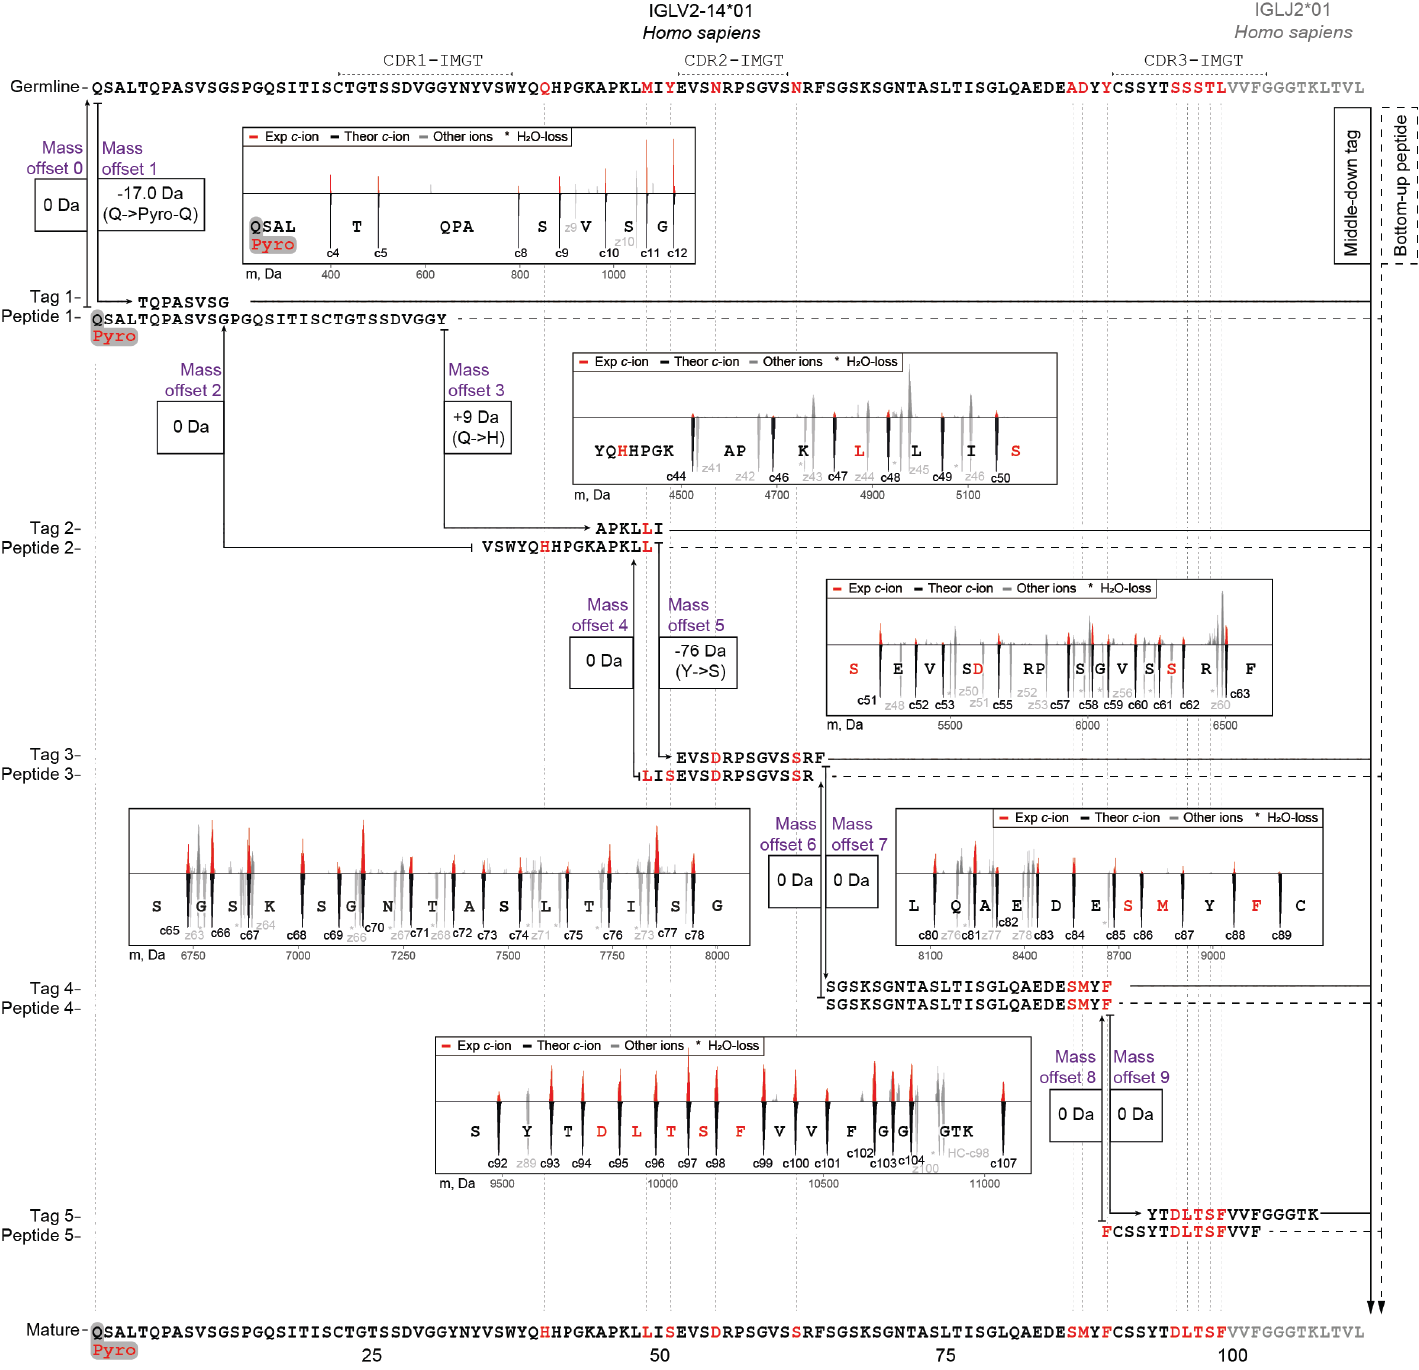
\includegraphics[]{Chapter.3/Figures/fs8.png}
    \caption{
      \textbf{Refining of the sequence of clone \textsuperscript{24.4} 1 \textsubscript{47359.4} light chain germline IGLV2-14$\star$01-IGLJ2$\star$01, based on the iterative integration of middle-down and bottom-up proteomics data.} ~~a) First, the sequence tags detected in the middle-down MS data were used as arrays of consecutive fragment peaks, which directly hinted at the presence of 11 mutations (M49L, Y51S, Y51S, N55D, N62S, A85S, D86M, Y88F, S95D, S96L, S97T, T98S, and L99F). Next, these tags were aligned to the \emph{de novo} sequenced peptide sequences obtained by bottom-up MS, revealing 2 additional mutations. The highest scoring aligned peptides were used to extend the initial sequence tags, and then these steps were iteratively repeated. At each step of tag extension, the mass offsets were calculated by comparing a mass gap between two consecutive tags to the mass of amino acid residues in the corresponding gap in the germline sequence. Iteratively, middle-down tags were extended with aligning peptides until all (if possible) mass offsets become equal to 0 Da. Eventually, 13 mutations and one modified residue (Pyro-Q) were determined for the \textsuperscript{24.4} 1 \textsubscript{47359.4} light chain sequence. De-charged isotopic distributions of the fragments involved in each sequence tag are displayed as red peaks in the corresponding insets with the theoretical isotopic distributions for these fragments displayed underneath each fragment. Fragmentation spectra of the peptides used in this refining process for the CDRs are shown in \textbf{\autoref{fig:fig3.5}}. See also \textbf{\autoref{tab:tabdummy3.5}}. for an overview of the evidence supporting each detected amino acid mutation.
    }
    \label{fig:figs3.8}
  \end{figure*}

  \vspace{1cm}

  \begin{figure*}[!ht]
    \center
    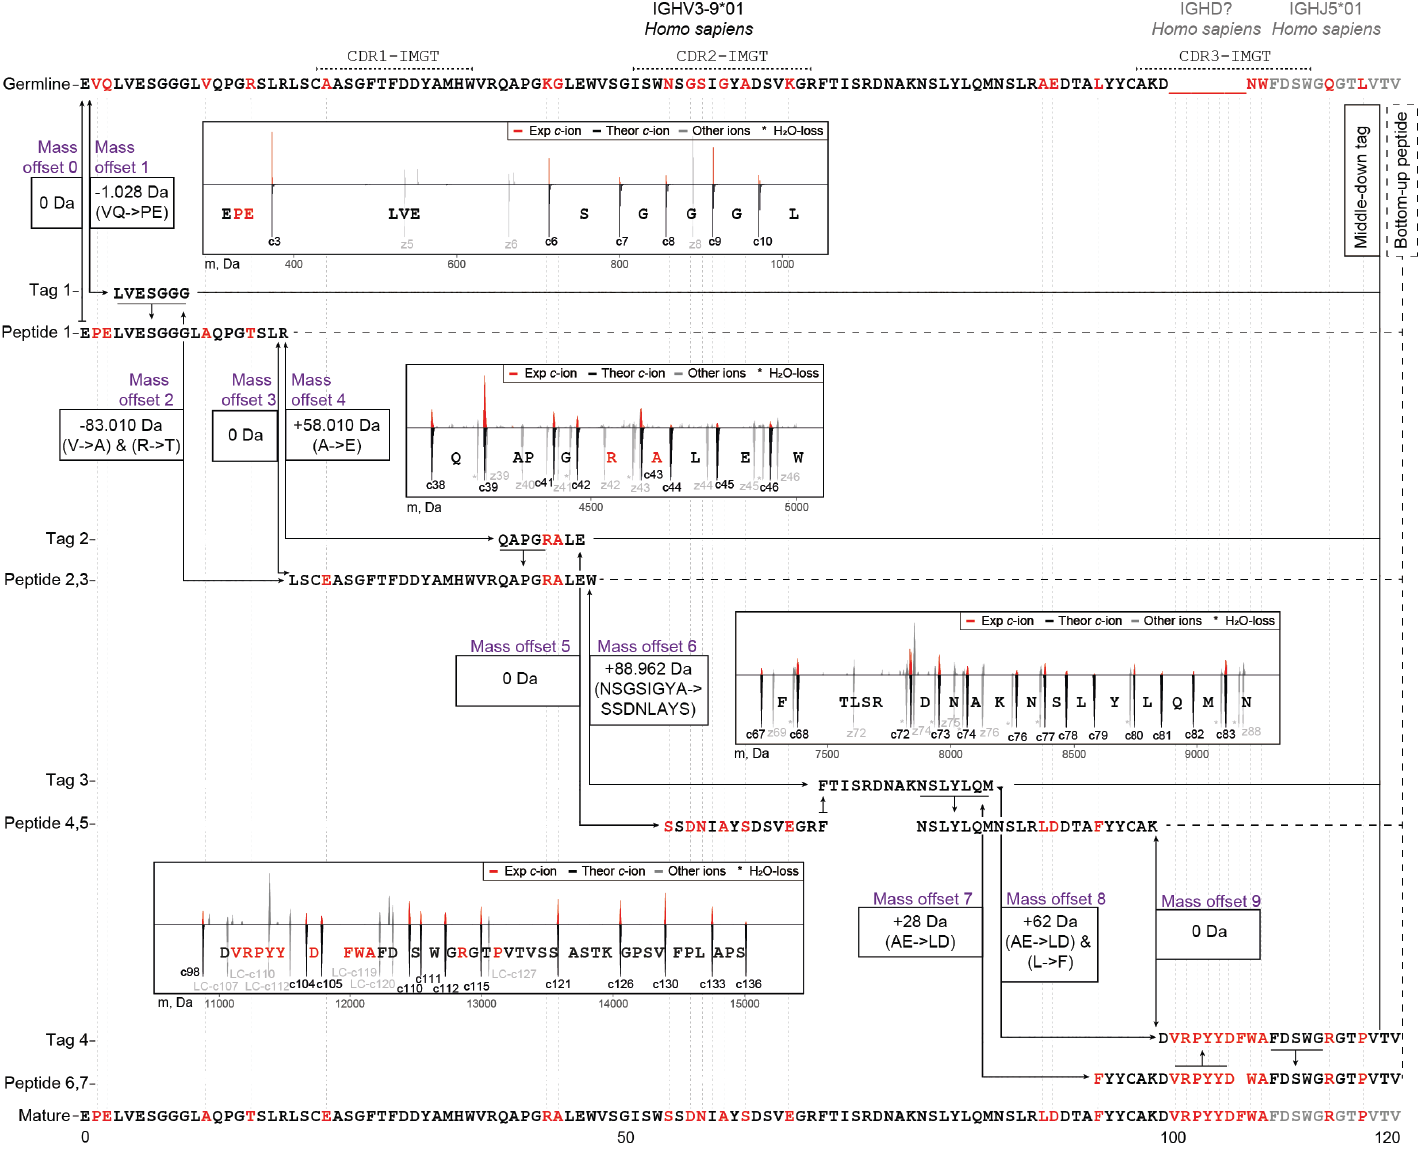
\includegraphics[]{Chapter.3/Figures/fs9.png}
    \caption{
      \textbf{Refining of the sequence of clone \textsuperscript{24.4} 1 \textsubscript{47359.4} heavy chain germline IGHV3-9$\star$01-IGHJ5$\star$01, based on the iterative integration of middle-down and bottom-up proteomics data.} ~~a) First, sequence tags were detected in the middle down MS data as arrays of consecutive fragment peaks similar to refining of the light chain. Next, these tags were aligned to the \emph{de novo} sequenced peptides from bottom-up MS. The highest-scoring aligned peptides were used to extend the initial tags, and then this step was repeated. At each step of tag extension, the mass offsets were calculated by comparing a mass gap between two consecutive tags to the mass of amino acid residues in the corresponding gap in the germline sequence. Iteratively, tags were extended with aligning peptides until all (if possible) mass offsets become equal to 0 Da. Eventually, more than 20 mutations were determined for the N-terminal portion of the heavy chain for clone \textsuperscript{24.4} 1 \textsubscript{47359.4}. De-charged isotopic distributions of the fragments involved in each sequence tag are displayed as red peaks in the corresponding insets with the theoretical isotopic distributions for these fragments displayed underneath each fragment. Fragmentation spectra of the peptides used in this refining process for the CDRs are shown in \textbf{\autoref{fig:fig3.5}}.
    }
    \label{fig:figs3.9}
  \end{figure*}

  \vspace{1cm}

  \begin{figure*}[!ht]
    \center
    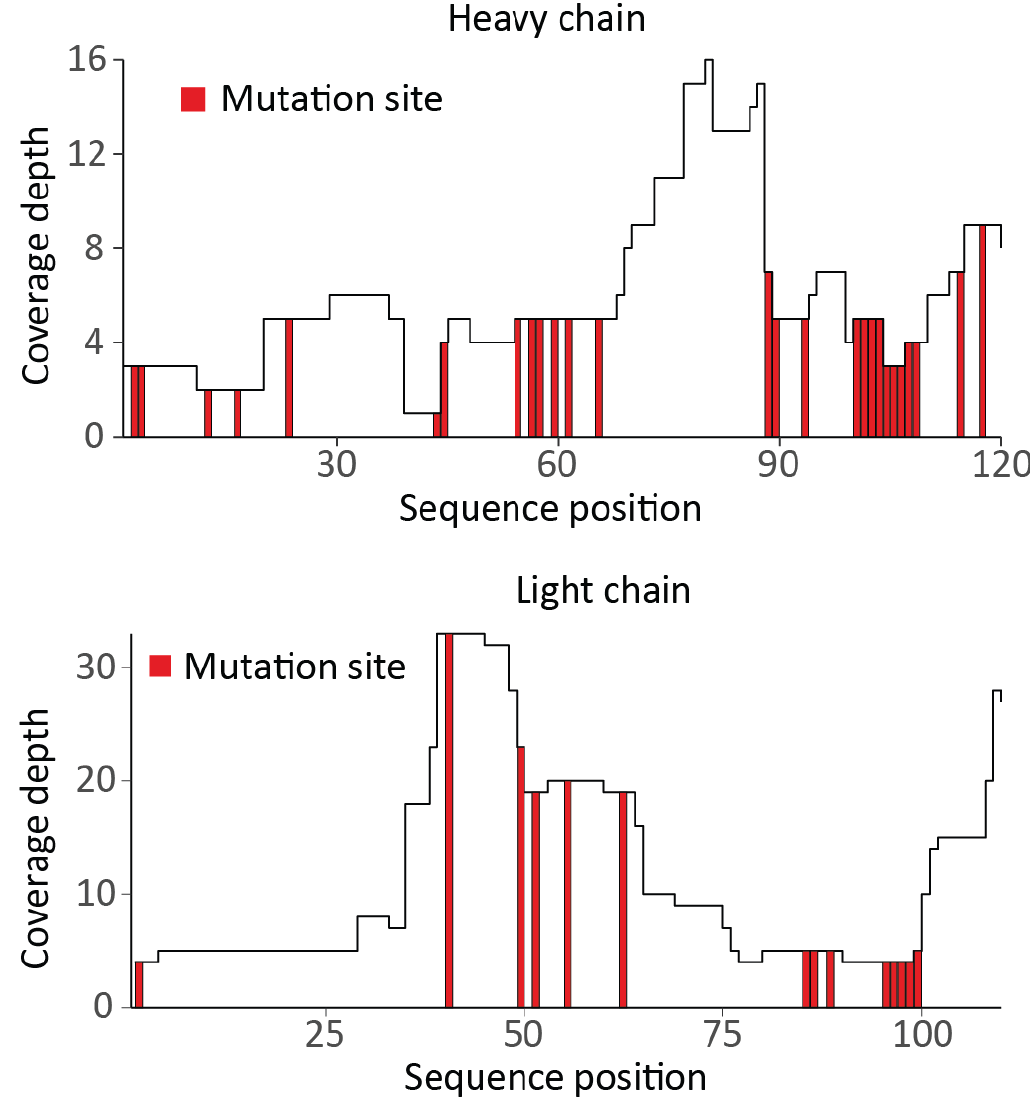
\includegraphics[]{Chapter.3/Figures/fs10.png}
    \caption{
      \textbf{Coverage depths for \emph{de novo} sequenced light and heavy chains of the clone \textsuperscript{24.4} 1 \textsubscript{47359.4} from donor F59.} ~~a) Values at each position represent the number of unique peptides identified in the bottom-up LC-MS/MS data. The determined mutation sites are depicted in red. Only the first 110 and 120 amino acids are shown for the light and heavy chain, respectively.
    }
    \label{fig:figs3.10}
  \end{figure*}

\end{subappendices}

\clearpage
\section*{References}
\bibliographystyle{Stylesettings/pnas}
\patchcmd{\thebibliography}
{\clubpenalty 4000\widowpenalty 4000}
{\clubpenalties 1 10000 \widowpenalties 1 10000}
{}{}
\bibliography{chapmerge}
\stopthumb


